\documentclass{article}

\usepackage{graphicx}
\usepackage{pdflscape}
\usepackage{afterpage}
\extrafloats{200}
\maxdeadcycles=1000
% if you need to pass options to natbib, use, e.g.:
%     \PassOptionsToPackage{numbers, compress}{natbib}
% before loading neurips_2021

% ready for submission
\usepackage[final]{neurips_2021}

% to compile a preprint version, e.g., for submission to arXiv, add add the
% [preprint] option:
%     \usepackage[preprint]{neurips_2021}

% to compile a camera-ready version, add the [final] option, e.g.:
%     \usepackage[final]{neurips_2021}

% to avoid loading the natbib package, add option nonatbib:
%    \usepackage[nonatbib]{neurips_2021}

\usepackage[utf8]{inputenc} % allow utf-8 input
\usepackage[T1]{fontenc}    % use 8-bit T1 fonts
\usepackage{hyperref}       % hyperlinks
\usepackage{url}            % simple URL typesetting
\usepackage{booktabs}       % professional-quality tables
\usepackage{amsfonts}       % blackboard math symbols
\usepackage{nicefrac}       % compact symbols for 1/2, etc.
\usepackage{microtype}      % microtypography
\usepackage{xcolor}         % colors

\title{Results from the deep learning challenge associated with the 3MD4040 lecture on plankton classification}

% The \author macro works with any number of authors. There are two commands
% used to separate the names and addresses of multiple authors: \And and \AND.
%
% Using \And between authors leaves it to LaTeX to determine where to break the
% lines. Using \AND forces a line break at that point. So, if LaTeX puts 3 of 4
% authors names on the first line, and the last on the second line, try using
% \AND instead of \And before the third author name.

\author{%
Jérémy Fix\\
\textit{LORIA, CNRS,} \\
\textit{Université de Lorraine, CentraleSupélec}\\
Gif-sur-Yvette, France \\
\texttt{jeremy.fix@centralesupelec.fr}
}

\begin{document}

\maketitle

\begin{abstract}
	This year, the deep learning lecture on the Metz campus of CentraleSupélec was evaluated by the participation to a custom challenge on plankton classification hosted on Kaggle. This
	paper presents the competition and the results obtained by the 13 "competing"
	teams. The challenge was hosted on kaggle \url{https://www.kaggle.com/c/3md4040-2022-challenge}.
\end{abstract}

\section{Context}

\subsection{Why a challenge}

I used to evaluate the deep learning lecture by a standard paper and pen exam. But I always thought that was not the best way to evaluate the students because deep learning is a know-how in addition to a theoretical understanding of the concepts. You cannot obtain reasonnable performance with your deep learning code if you do not understand what is going on. There are so many degrees of freedom that a random exploration of the hyperparameters is hopeless.

The challenge lasted approximately 2 months, started in December 2021 and ended beginning of February 2022.

\subsection{Grading}

Grading of the students' contributions is on three topics :
\begin{itemize}
	\item the performance on the leaderboard for 5 points
	\item the quality of the 20 minutes long video recorded presentation for 5 points
	\item the quality of the code and experimentations for 10 points
\end{itemize}

I once asked orally to provide a little article presenting the experimental track but forgot to mention it on the grading page and therefore did not ask for it at the end of the challenge.

For the performance on the leaderboard, the points were allocated as~:
\begin{itemize}
	\item 1 point if the submitted predictor performs better than a benchmark linear network
	\item 2 points if the submitted predictor performas better than a benchmark basic CNN network
	\item 2 points if the submitted predictor ranks first
\end{itemize}

\subsection{Rules}

The students were asked to respect the following rules :
\begin{itemize}
	\item the predictor must be a neural network
	\item the code must be in pytorch. Using higher level framework such as pytorch lightning was allowed
	\item the students were not allowed to share codes between the teams
	\item the students were allowed and strongly encouraged to ask questions on a dedicated forum and they would be provided hints under the condition that the previous rules were not violated
\end{itemize}

In practice, video sessions were organized with the groups that had the most difficulties to come into the challenge.


%-----------------------------------------------------------------------------------
\section{The challenge on plankton classification}

The data for the challenge come from the ZooScanNet dataset (\url{https://www.seanoe.org/data/00446/55741/}). It contains 1,433,278 images sorted in 93 taxa. We only used the images and not the native nor skimage features that were provided. It does not mean that these handcrafted features could not be useful for plankton classification, it is just the the challenge focused exclusively on image classifcation (but definitely, a later issue should include them).

\subsection{Data preparation}

Three folds were prepared from the original data :
\begin{itemize}
	\item a training set of 855.394 images
	\item a public test set of 47.473 images
	\item a private test set of 47.472 images
\end{itemize}

We did not kept all the classes from the original 93 taxa. Five classes were ignored : \emph{badfocus\_artefact}, \emph{badfocus\_Copepoda}, \emph{bubble}, \emph{multiple\_\_Copepoda} and \emph{multiple\_\_other}. Three classes were fused : \emph{detritus}, \emph{fiber\_\_detritus} and \emph{seaweed}. Therefore, at the end, we get a total of $86$ classes. We also kept a maximum of $200.000$ per classes (before merging classes which explains why the detritus has more than $200000$ samples).

One concern in preparing the data challenge is to prevent cheating such as overfitting the original dataset (which then comprise the test data). To prevent the challengers from cheating, a random rotation was applied to the image.


\subsection{Data statistics}

All the sets were identically balanced, i.e. the classes are imbalanced but imbalanced in the same proportions irrespectively of the fold. After the challenge, rereading the different classes, it might have been worth fusing artefact with detritus, and also maybe some egg classes. There are also two classes for tail and head which might gather tails and heads of different species which in no way can be considered as a single class. These two classes should have probably been discarded.

\begin{figure}
	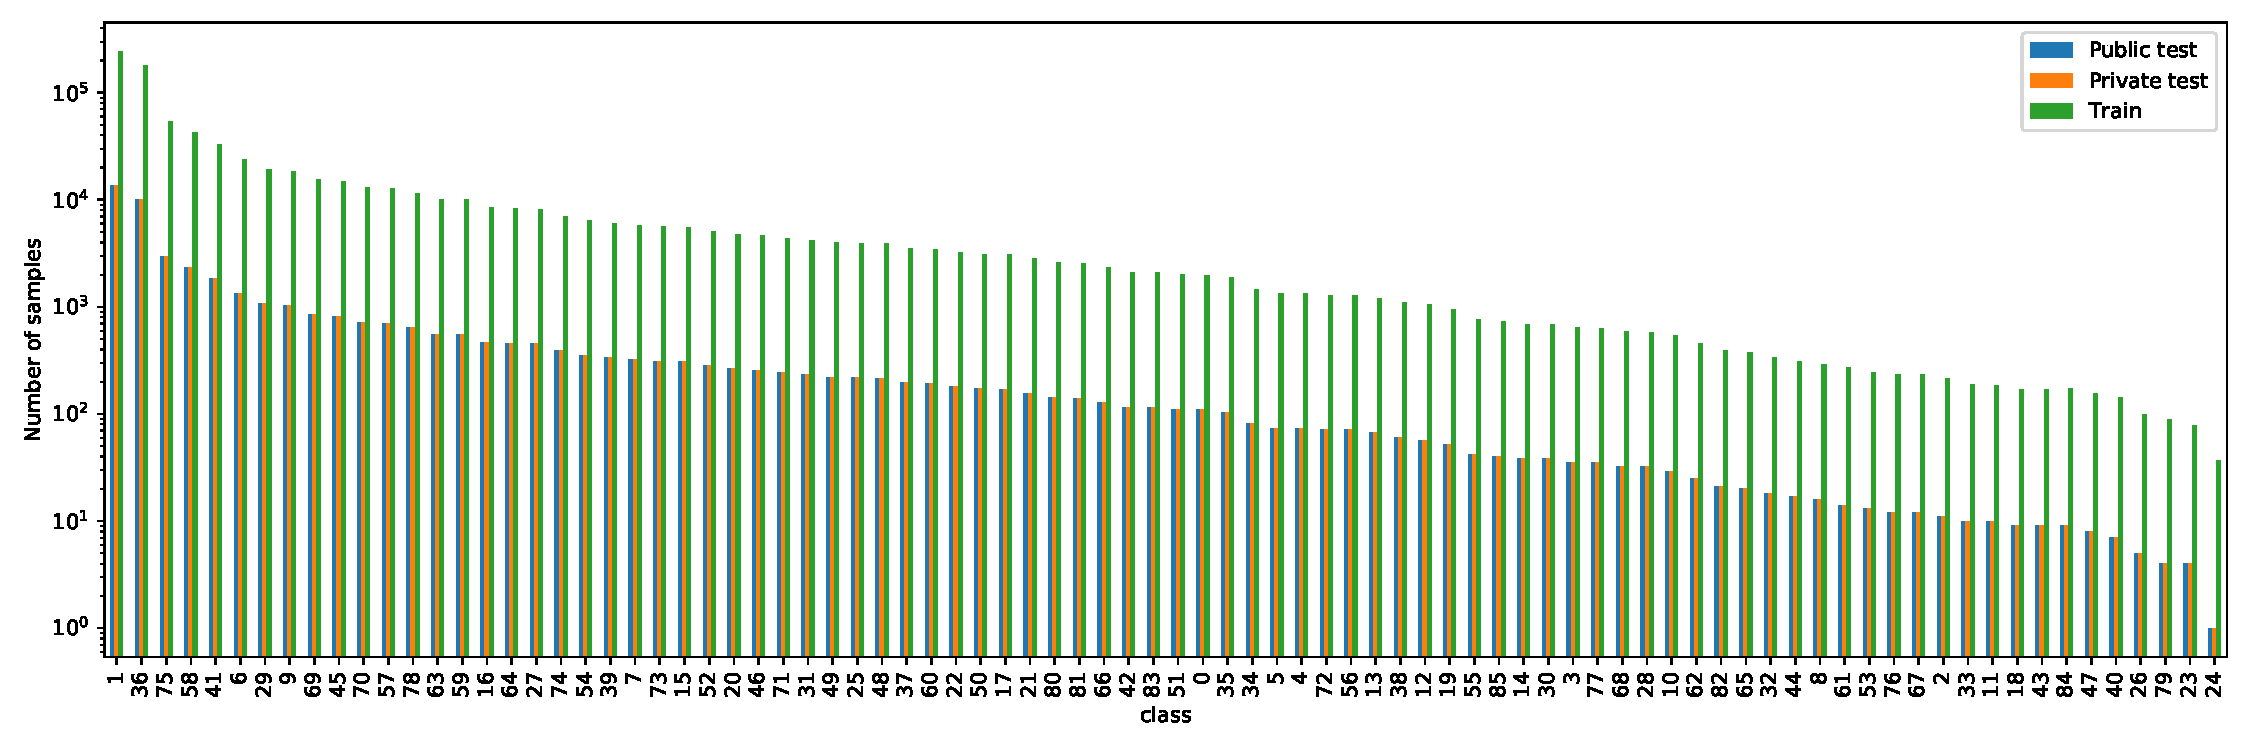
\includegraphics[width=\columnwidth]{figs/stats.pdf}
	\caption{\label{fig:classdistrib} The distribution of samples per classes. See the appendix for the details, especially the class names}
\end{figure}

The distribution of the samples over the different folds is shown on figure~\ref{fig:classdistrib}. The dataset is imbalanced and that was one interest of the challenge. The class with the most samples is the detritus followed by the Calanoida. The class with the lowest number of samples is the Ctenophora which has only $36$ samples in the training set and $1$ sample in both the public and private test sets.

The images vary in size. During the prepation of the dataset, the images were resized so that their height and width do not exceed $300$, keeping their aspect ratio. Athough the original images vary in sizes, this choice was made to keep the weight of the whole dataset reasonnable. Note however that this choice may have introduced difficulties in the recognition process (which could have been mitigated by providing the handcrafted features). Indeed, this resize erases class specific shape distributions. The distribution of heights and widhts of the datasets are shown on figure~\ref{fig:sizes}, left for the training set, \ref{fig:sizes}, middle for the test set and \ref{fig:sizes}, right for the original images. For practical simplicity, only the size plot of the training set indicates the class belongings.


\begin{figure}
	\begin{center}
		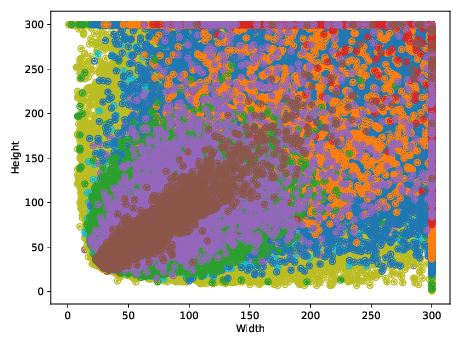
\includegraphics[width=0.3\columnwidth]{figs/size_train.png}
		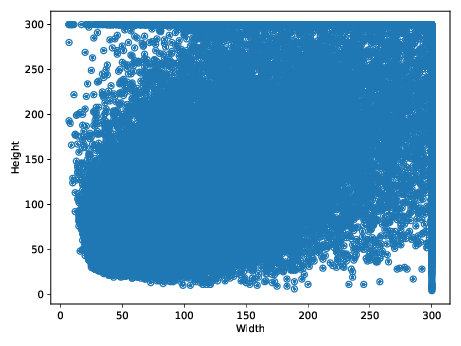
\includegraphics[width=0.3\columnwidth]{figs/sizes_test.png}
		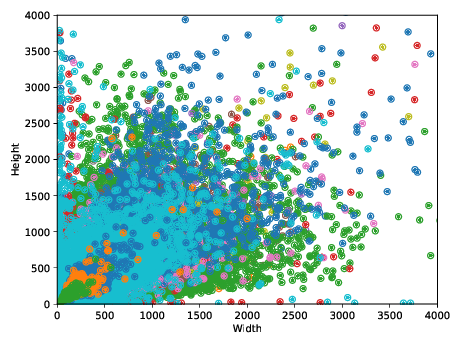
\includegraphics[width=0.3\columnwidth]{figs/size_orig.png}
	\end{center}
	\caption{\label{fig:sizes} Distribution of the image sizes for the training set (left), test set(right) and the original dataset (right). On the plot on the right, the original sizes have been limited to $4000$ for both widths and heights but there exists outliers up to $10000$ in width or $12000$ in height.}
\end{figure}

%TODO: Plot size distribution as a 2D scatter plot

\subsection{Evaluation metrics}

The challenge is a classification challenge with strongly imbalanced classes. The competitors were evaluated with the macro-average F1 score which is the average of the class F1 scores.

The class F1 score is defined as the harmonic mean of the precision and recall. Given a class $k$, the number of true positives $TP_k$, false positive $FP_k$, and false negatives $FN_k$, precision, recall and $F1$ are computed as~:
\begin{eqnarray*}
	precision_k &=& \frac{TP_k}{TP_k + FP_k}\\
	recall_k &=& \frac{TP_j}{TP_k + FN_k}\\
	\frac{1}{F1_k} &=& \frac{1}{2}(\frac{1}{precision_k} + \frac{1}{recall_k})
\end{eqnarray*}

The macro-average F1 is then defined as the average of all the classes~:

\begin{equation}
	\mbox{macro-F1} = \frac{1}{86}\sum_{k=0}^{85} F1_k
\end{equation}

%-----------------------------------------------------------------------------------
\section{The submissions of the participants}

In the next section, we give a quick overview of the different techniques involved by the participants for the different topics of : 

\begin{itemize}
	\item data loading 
	\item data augmentation
	\item classification model architectures
	\item optimization setup (optimizer, scheduler, ..)
	\item handling of the class imbalance
\end{itemize}

That overview is built from inspection of the submitted codes and may not reflect all the configurations that have been tested by the participants. The collected information from the code are summarized in tables~\ref{table:overview1},\ref{table:overview2},\ref{table:overview3}.

\afterpage{
	\clearpage
	\thispagestyle{empty}
	\begin{landscape}
		\begin{table}
			\begin{tabular}{p{3cm}|p{3cm}|p{3cm}|p{3cm}|p{3cm}|p{3cm}|p{3cm}}
			Participant & Data preprocessing & Train augmentation & Test augmentation & Model architectures & Optimizer and scheduler & Class imbalance \\
			\hline
			SpongeBob & 
			Resize($224$), Normalize($0.5$, $0.5$) & 
			HFlip($0.5$), VFlip($0.5$) , Rotate($-40, 40$), Translate($0.3, 0.5)$, Scale($0.7, 1.3$), Shear($-30, 30$)&
			None &
			Custom ConvNet, Pretrained torchvision ResNet, AlexNet, DenseNet121, timm ViT, EfficientNetB2, ConvNeXt, RegNetx\_320, EfficientNetv2\_rw\_t, BeIT, CoaT&
			Cross Entropy loss, Adam(lr=$5e-4$), ReduceLROnPlateau(validation loss), early stopping on validation F1, Batch size $64$,  Random train/valid split ($0.95, 0.05$)&
			Class weights in the CE loss\\
			\hline
			DeepWhale & 
			Pad/Resize($224$), ImageNet normalization&
			HFlip($0.5$), VFlip($0.5$), Rotate($-150, 150$)&
			None& 
			Custom CNN, pretrained ResNet50, 101, 152, VGG19, SqueezeNet from torchvision&
			Cross EntropyLoss, SGD($1e-3$), ReduceLROnPlateau(validation loss), early stopping on the validation loss, batch size $32$, train/valid split ($0.8, 0.2$) per class &
			batch sampler with $f_k = 1/count_k$\\
			\hline
			GrandeRegazzoni & 
			SquarePad($300$) or ResizeCrop($128$) or Resize($150$)&
			HFlip($0.5$), VFlip($0.5$), Rotate($-40, 40$), Translate($-0.2, 0.2$)&
			None&
			Custom ConvNet, EfficientNet\footnote{\url{https://github.com/lukemelas/EfficientNet-PyTorch}}, HRNet, ResNet, SwinTransformer&
			Cross Entropy loss, Adam($1e-3$), ReduceLROnPlateau(validation F1), early stopping on the validation loss, Batch size $128$, train/valid split ($0.8, 0.2$) per class &
			batch sampler with $f_k = 1/count_k$\\
			\hline
			Voleurs d'huile&
			Resize($224$), z-score normalization by training mean/std&
			HFlip($0.5$), VFlip($0.5$), Gaussian Blur&
			None&
			Custom CNN, pretrained torchvision ResNet and DenseNet121 & 
			Cross Entropy loss, Adam($4e-4$), StepLR($\gamma=0.1, step=6$), early stopping on the validation loss, Batch size $32$, train/valid split ($0.8, 0.2$) &
			None\\
			\hline
		\end{tabular}
			\caption{Overview of the experiments of the participants. Part 1. \label{table:overview1}}
	\end{table}

		\begin{table}
			\begin{tabular}{p{3cm}|p{3cm}|p{3cm}|p{3cm}|p{3cm}|p{3cm}|p{3cm}}
			Participant & Data preprocessing & Train augmentation & Test augmentation & Model architectures & Optimizer and scheduler & Class imbalance \\
			\hline
			Metz Dream Deep & 
			Resize($224$), Normalize($0.5$, $0.5$) & 
				Rotate($0, 360$), HFlip($0.5$), Translate($0.2$), Normalization$(0.5, 0.5$)&
			None&
			&
				Cross entropy loss, Adam($1e-4$), Weight decay $1e-4$, ..., batch size $128$, train/valid split&
			batch sampler $f_k=1/count_k$\\
			\hline
			The Backpropagated StuBBorns & 
			Resize($224$), Normalize($0.5$, $0.5$) & 
			&
			&
			&
			&
			\\
			\hline
			JMBmc & 
			Resize($224$), Normalize($0.5$, $0.5$) & 
			&
			&
			&
			&
			\\
			\hline
			AG0D & 
			Resize($224$), Normalize($0.5$, $0.5$) & 
			&
			&
			&
			&
			\\
			\hline
		\end{tabular}
			\caption{Overview of the experiments of the participants. Part 2. \label{table:overview2}}
	\end{table}

		\begin{table}
			\begin{tabular}{p{3cm}|p{3cm}|p{3cm}|p{3cm}|p{3cm}|p{3cm}|p{3cm}}
			Participant & Data preprocessing & Train augmentation & Test augmentation & Model architectures & Optimizer and scheduler & Class imbalance \\
			\hline
			ResMetz & 
			Resize($224$), Normalize($0.5$, $0.5$) & 
			&
			&
			&
			&
			\\
			\hline
			CelestineFeuillat & 
			Resize($224$), Normalize($0.5$, $0.5$) & 
			&
			&
			&
			&
			\\
			\hline
			LesJongleurs & 
			Resize($224$), Normalize($0.5$, $0.5$) & 
			&
			&
			&
			&
			\\
			\hline
			DeepBeru4s & 
			Resize($224$), Normalize($0.5$, $0.5$) & 
			&
			&
			&
			&
			\\
			\hline
			The Whale Sharks & 
			Resize($224$), Normalize($0.5$, $0.5$) & 
			&
			&
			&
			&
			\\
		\end{tabular}
			\caption{Overview of the experiments of the participants. Part 3. \label{table:overview3}}
	\end{table}
	\end{landscape}
	\clearpage
}

Some of the participants also considered model averaging :

SpongeBox , GrandeRegazzoni (convenet, hrnet, efficientnet)

%TODO :Verifier le cout du padding : Fill value ?? 0.0 par défaut mais pour du blanc c'est 1.0 ?!

\subsection{The scores of the participants through time}

I find it interesting to see how the submissions of the participants improved through time. The teams submitted from 5 to 79 entries and the scores they obtained on the public and private test sets are shown on figure~\ref{fig:F1scores}.

\begin{figure}
	\begin{center}
		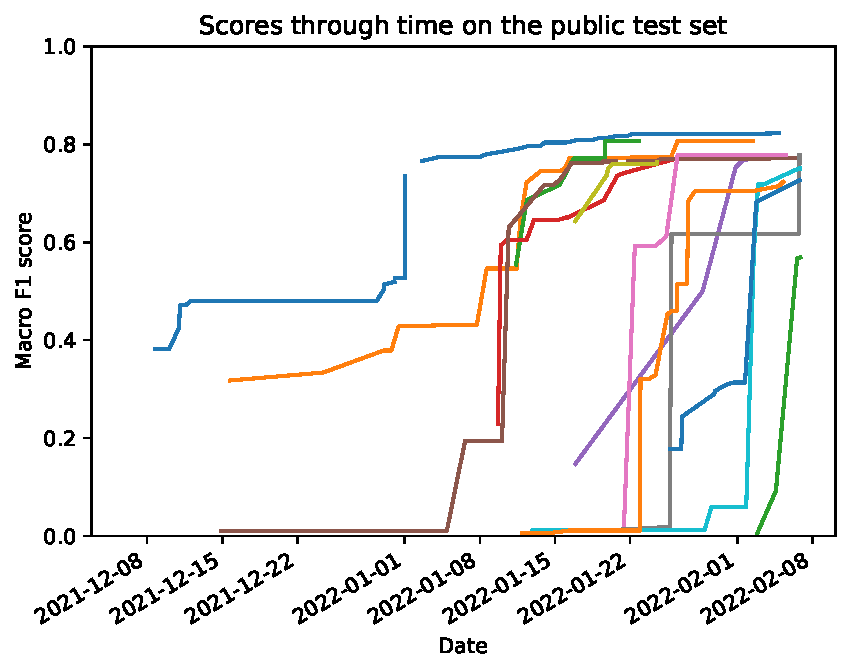
\includegraphics[width=0.45\columnwidth]{figs/public-test.pdf}
		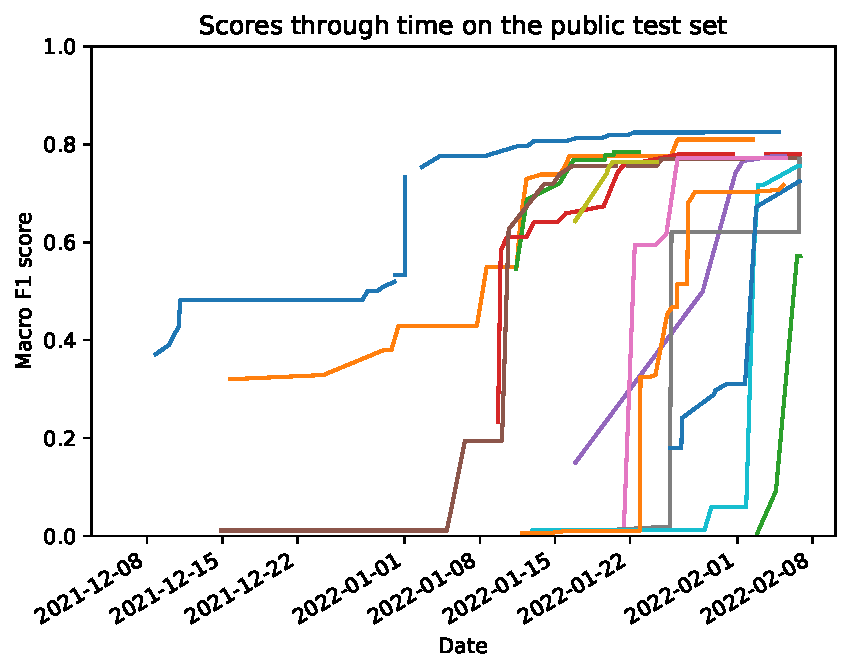
\includegraphics[width=0.45\columnwidth]{figs/private-test.pdf}
	\end{center}
	\caption{\label{fig:F1scores} Macro F1 on the public (left) and private (right) test sets as a function of time.}
\end{figure}

\subsection{Analysis of the results}

The best entries of all the teams ranged from 0.71 to 0.82 (except one outlier at 0.57) on the private leaderboard in macro average F1 score. The class F1 scores, computed from the whole test data (public and private) is displayed on figure~\ref{fig:class_f1_scores}, left. This graph displays the distribution of class F1 scores for each team, where the teams are ordered by decreasing macro average F1.

\begin{figure}
	\begin{center}
		\raisebox{-0.5\height}{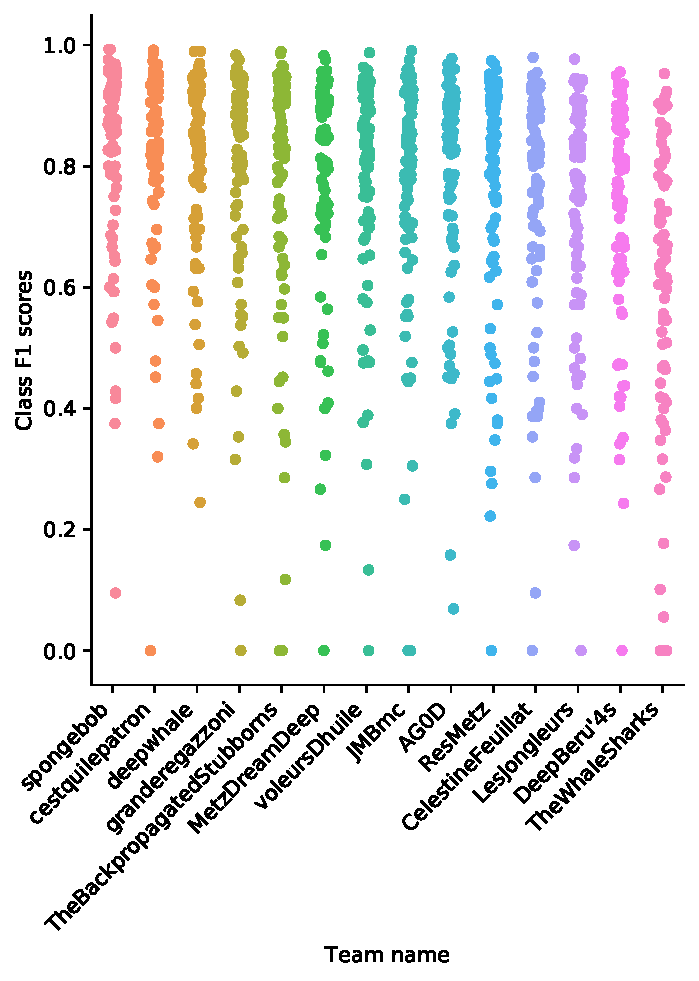
\includegraphics[width=0.25\columnwidth]{figs/class_f1_scores_per_team.pdf}}
		\hspace*{.4in}
		\raisebox{-0.5\height}{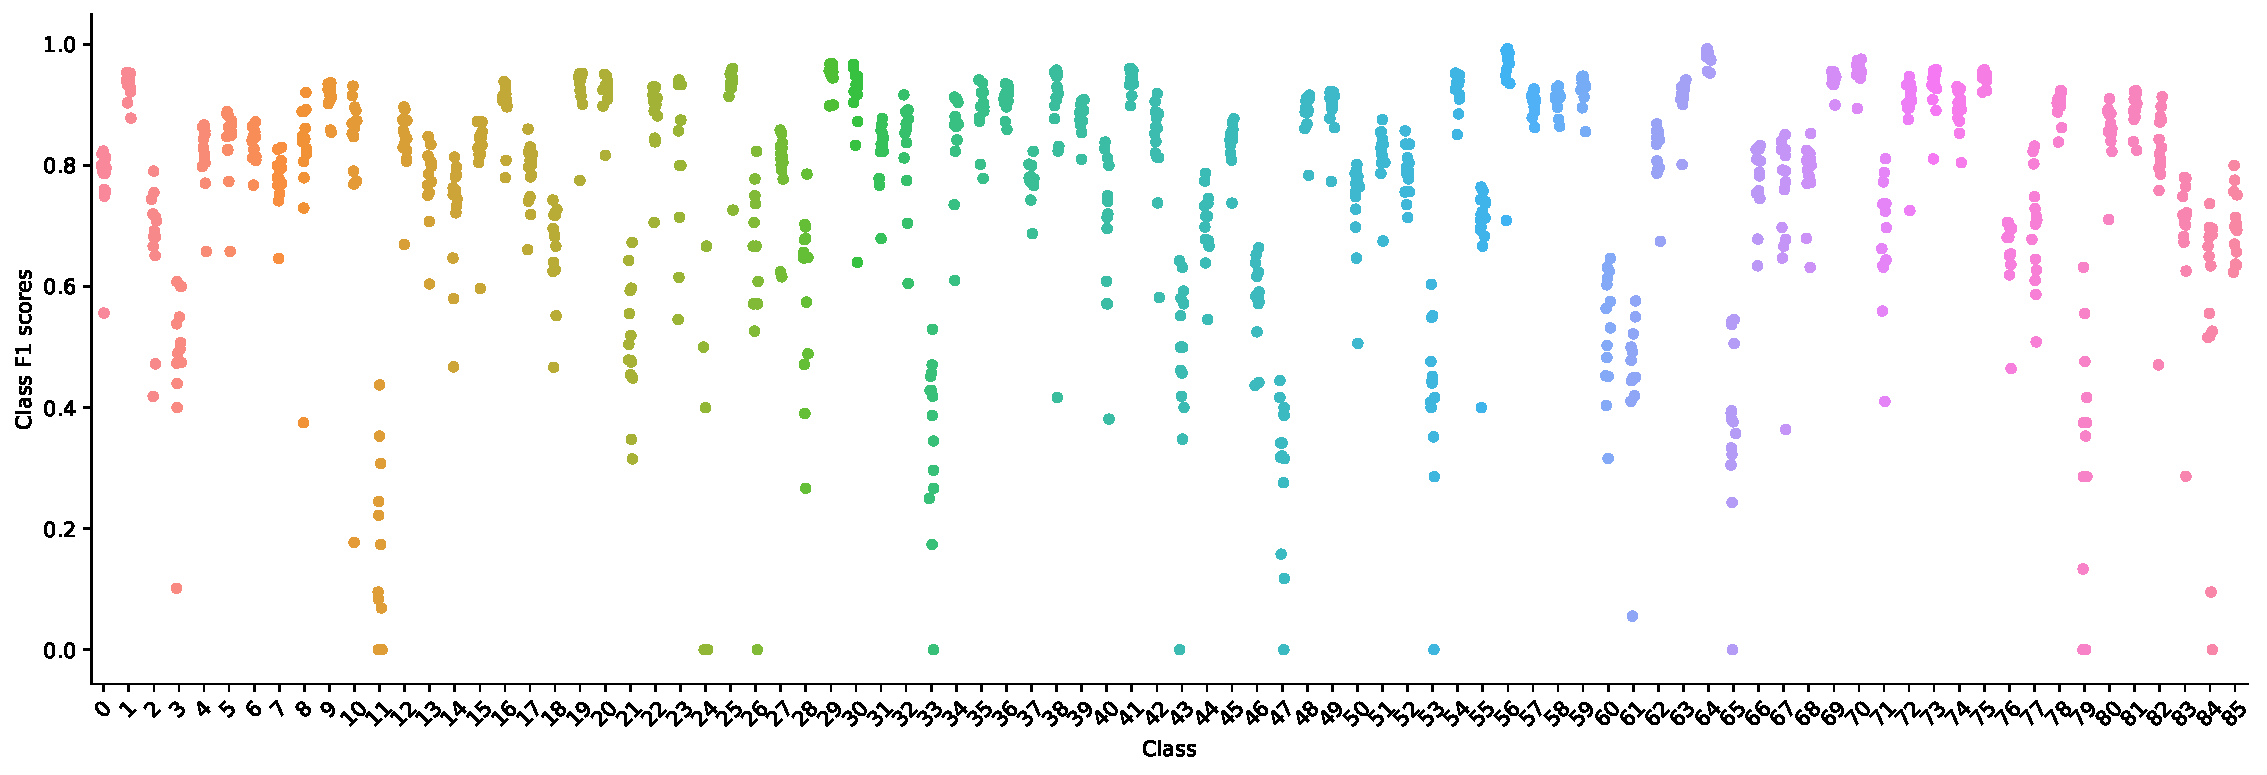
\includegraphics[width=0.62\columnwidth]{figs/class_f1_scores_per_class.pdf}}
	\end{center}
	\caption{\label{fig:class_f1_scores} Class F1 scores on the test data per team (left) and per class (right).}
\end{figure}

We can also plot the F1 scores from the class perspective rather than a team perspective. That view of the class F1 scores is shown on figure~\ref{fig:class_f1_scores}, right. This graph plots the distribution of the teams' F1 for every class. From this graph, we see that some classes are consistently well predicted (e.g. the classes $0$, $1$, $2$, $3$, $4$ and $6$) and some classes seem much harder to classify ($80$, $76$, $75$, $70$, $66$). In order to get an idea of the classes that appear to be the easiest to predict, we selected from the distribution of F1 scores, the classes for which the minimal F1 over all the teams is higher than 0.8 This choice leads to the easiest classes given in table~\ref{table:best_predicted}.


\begin{table}
\begin{tabular}{|l|r|}
Class names & Minimal F1 over all the teams \\
        \hline
1 detritus & 0.88\\ 
9 Oikopleuridae & 0.85\\ 
20 Brachyura & 0.82\\ 
29 Evadne & 0.90\\ 
36 Calanoida & 0.86\\ 
39 Noctiluca & 0.81\\ 
41 Chaetognatha & 0.90\\ 
54 Penilia & 0.85\\ 
57 Coscinodiscus & 0.86\\ 
58 Acartiidae & 0.86\\ 
59 Corycaeidae & 0.86\\ 
63 Limacinidae & 0.80\\ 
64 cyphonaute & 0.95\\ 
69 Phaeodaria & 0.90\\ 
70 Ostracoda & 0.89\\ 
73 nauplii Cirripedia & 0.81\\ 
74 Salpida & 0.80\\ 
75 Oithonidae & 0.92\\ 
78 Oncaeidae & 0.84\\ 
81 Cavoliniidae & 0.83
\end{tabular}
\caption{\label{table:best_predicted} The classes for which the minimal F1 score obtained by all the teams is above
$0.8$.}
\end{table}
                

In order to get an idea of the classes that appear to be the most difficult to predict, we selected from the distribution of F1 scores, the classes for which the maximal F1 over all the teams is smaller than 0.6. This choice leads to the hardest classes given in table~\ref{table:worst_predicted}.


\begin{table}
\begin{tabular}{|l|r|}
Class names & Maximal F1 over all the teams \\
        \hline
11 zoea Galatheidae & 0.44\\ 
33 nectophore Abylopsistetragona & 0.53\\ 
47 Euchirella & 0.44\\ 
61 cirrus & 0.58\\ 
65 part Copepoda & 0.55
\end{tabular}
\caption{\label{table:worst_predicted} The classes for which the maximal F1 score obtained by all the teams is below $0.6$.}
\end{table}
                

The last analysis we provide is the construction of the confusion matrices for all the participants. These are given in figures~\ref{fig:confusion}. Note the confusion matrices have been row normalized and the figures should be understood as the fraction of a given class that has been classified as such or such class.

\begin{figure}
	\begin{tabular}{ccccc}
		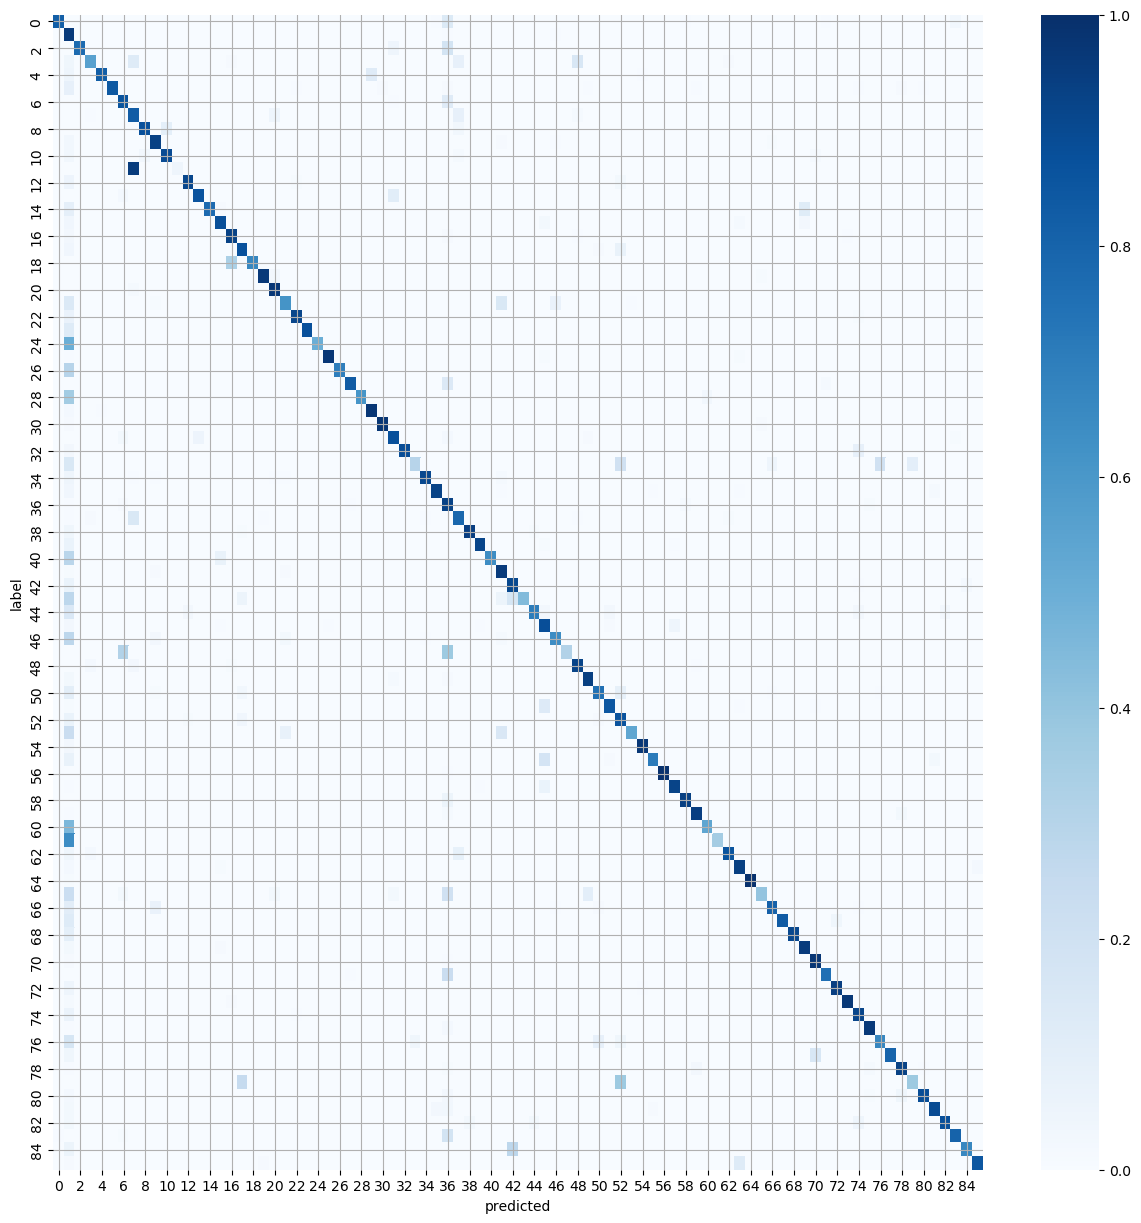
\includegraphics[width=0.18\columnwidth]{figs/confusion_matrix_spongebob.png}&
		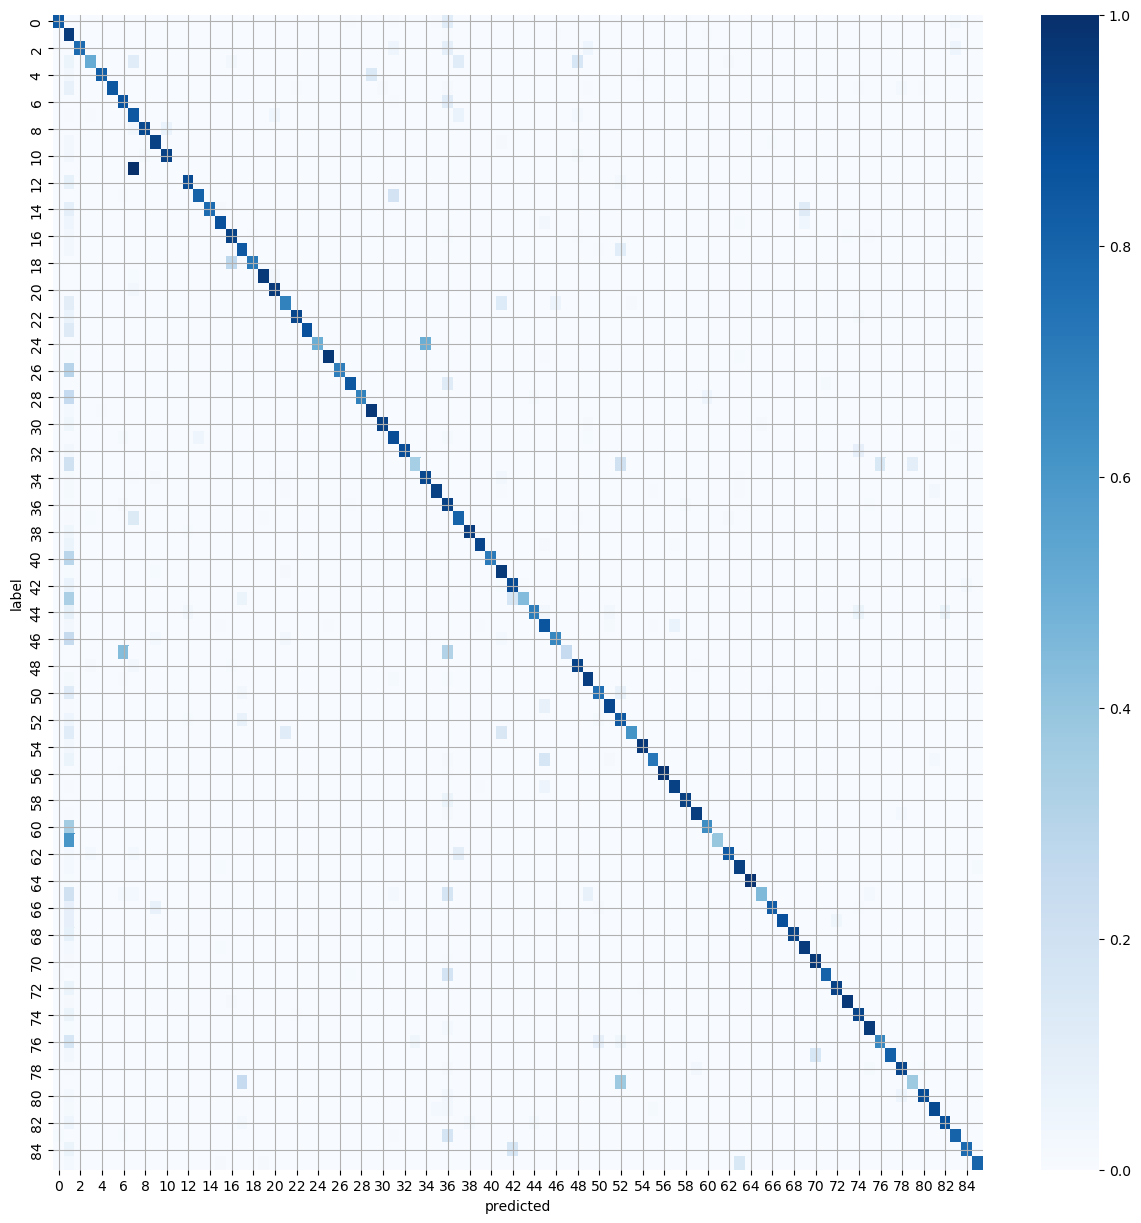
\includegraphics[width=0.18\columnwidth]{figs/confusion_matrix_cestquilepatron.png}&
		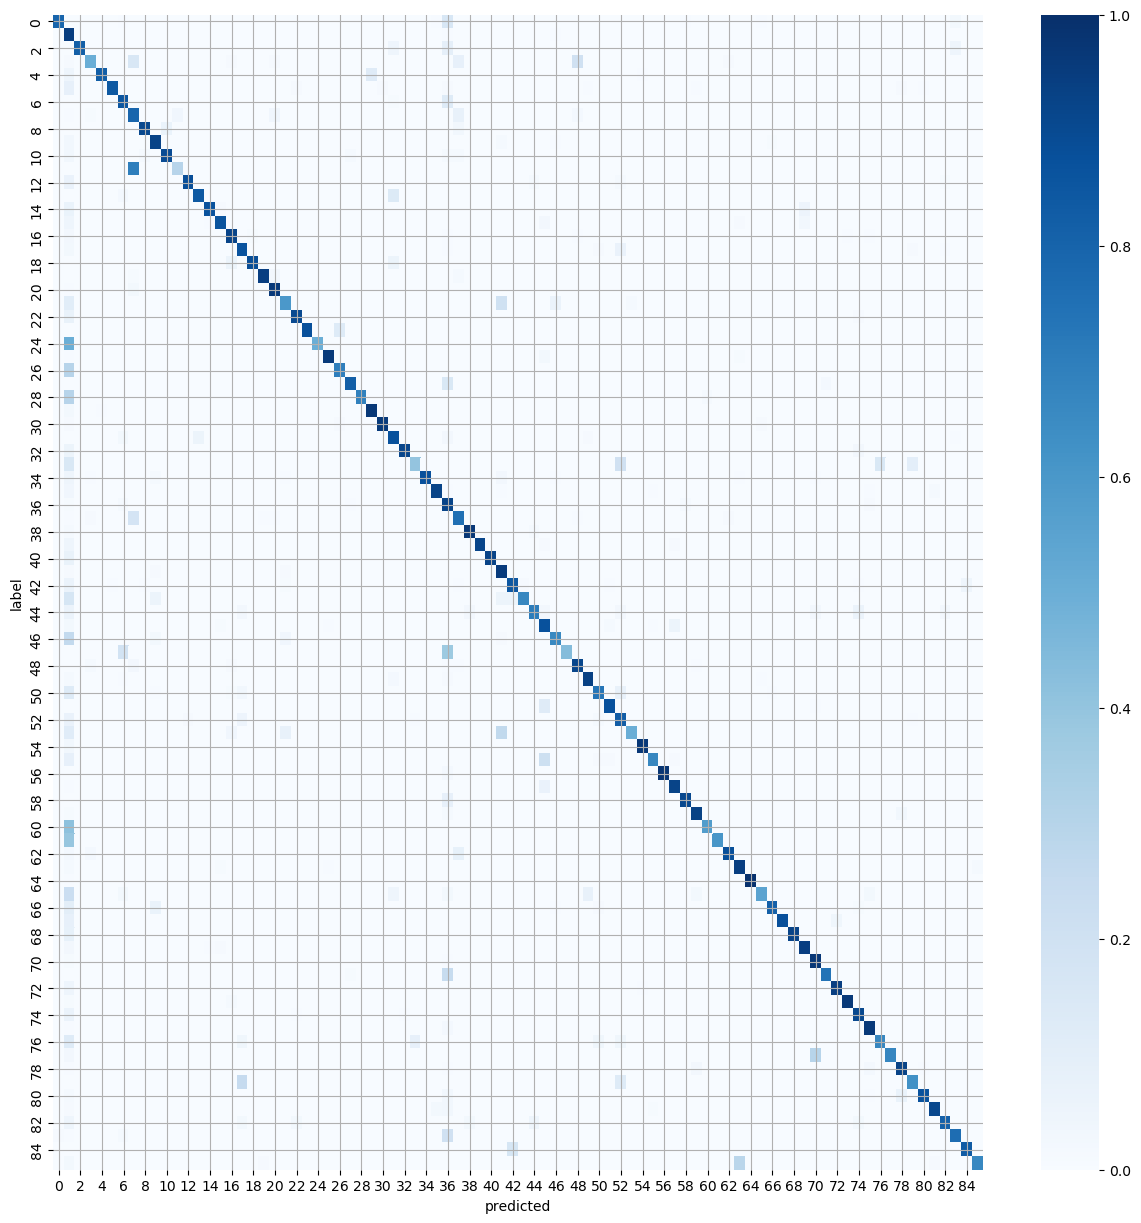
\includegraphics[width=0.18\columnwidth]{figs/confusion_matrix_deepwhale.png}&
		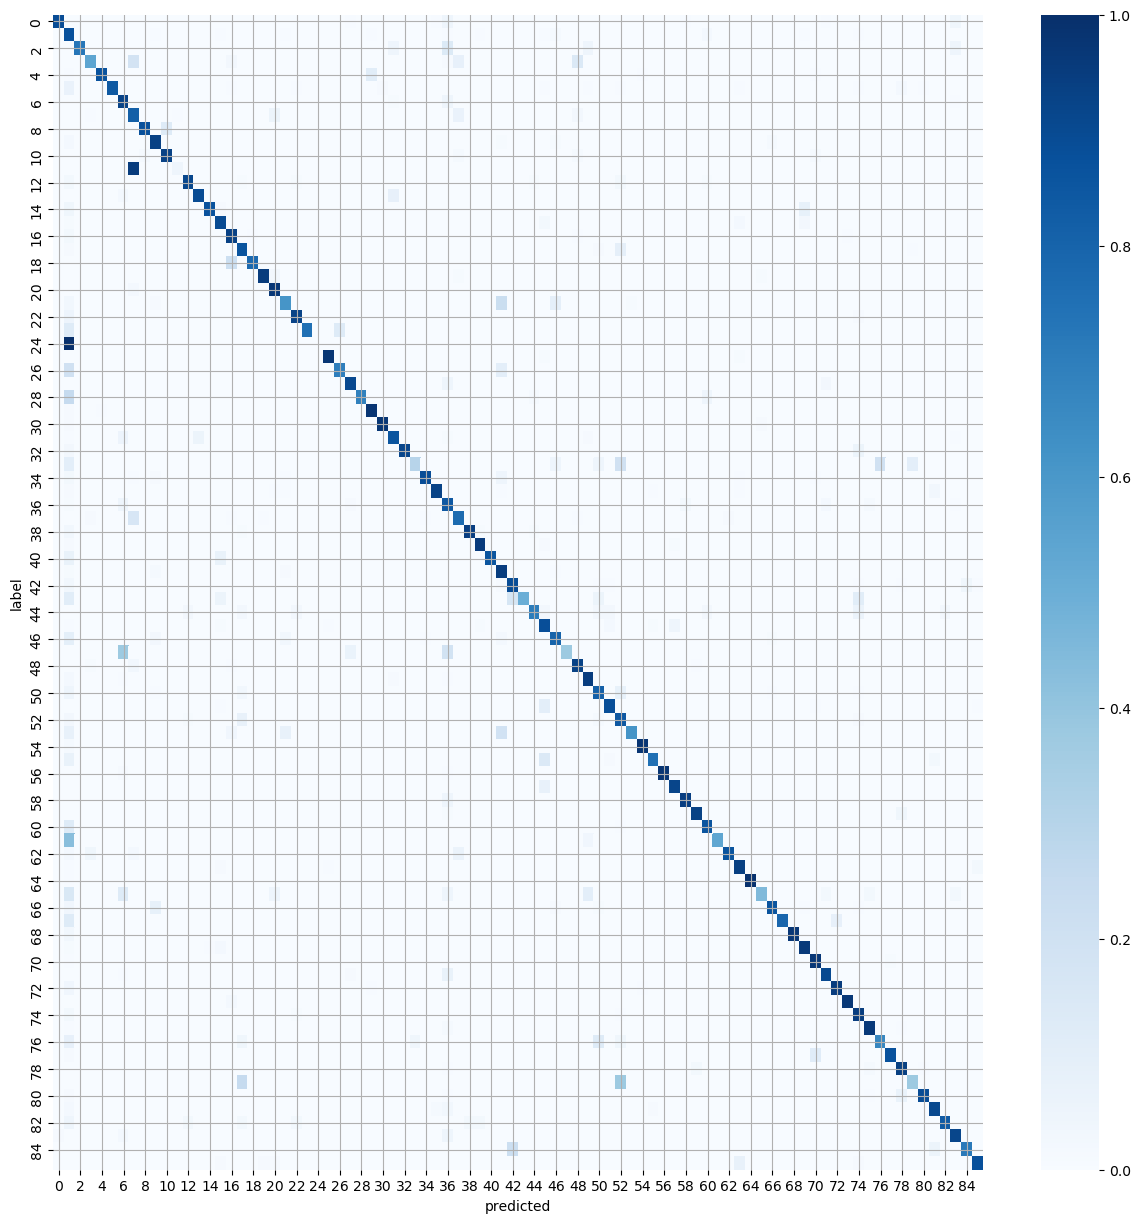
\includegraphics[width=0.18\columnwidth]{figs/confusion_matrix_granderegazzoni.png}&
        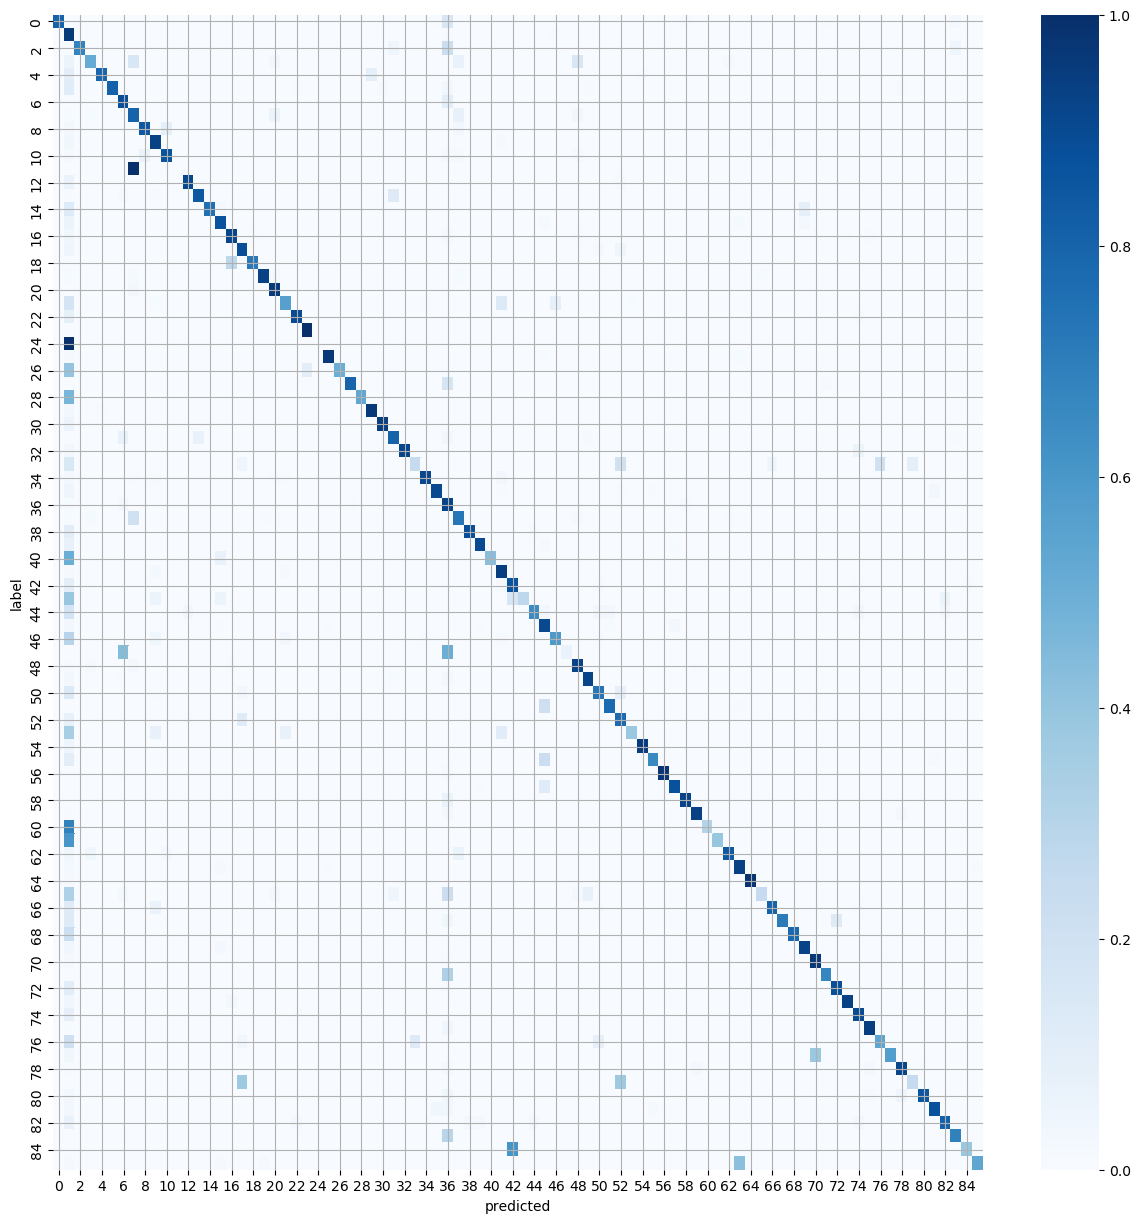
\includegraphics[width=0.18\columnwidth]{figs/confusion_matrix_TheBackpropagatedStubborns.png}\\
		SpongeBob & C'est qui l'patron & DeepWhalfigs/e & GrandeRegazzoni & The Backpropagated Stubborns\\
		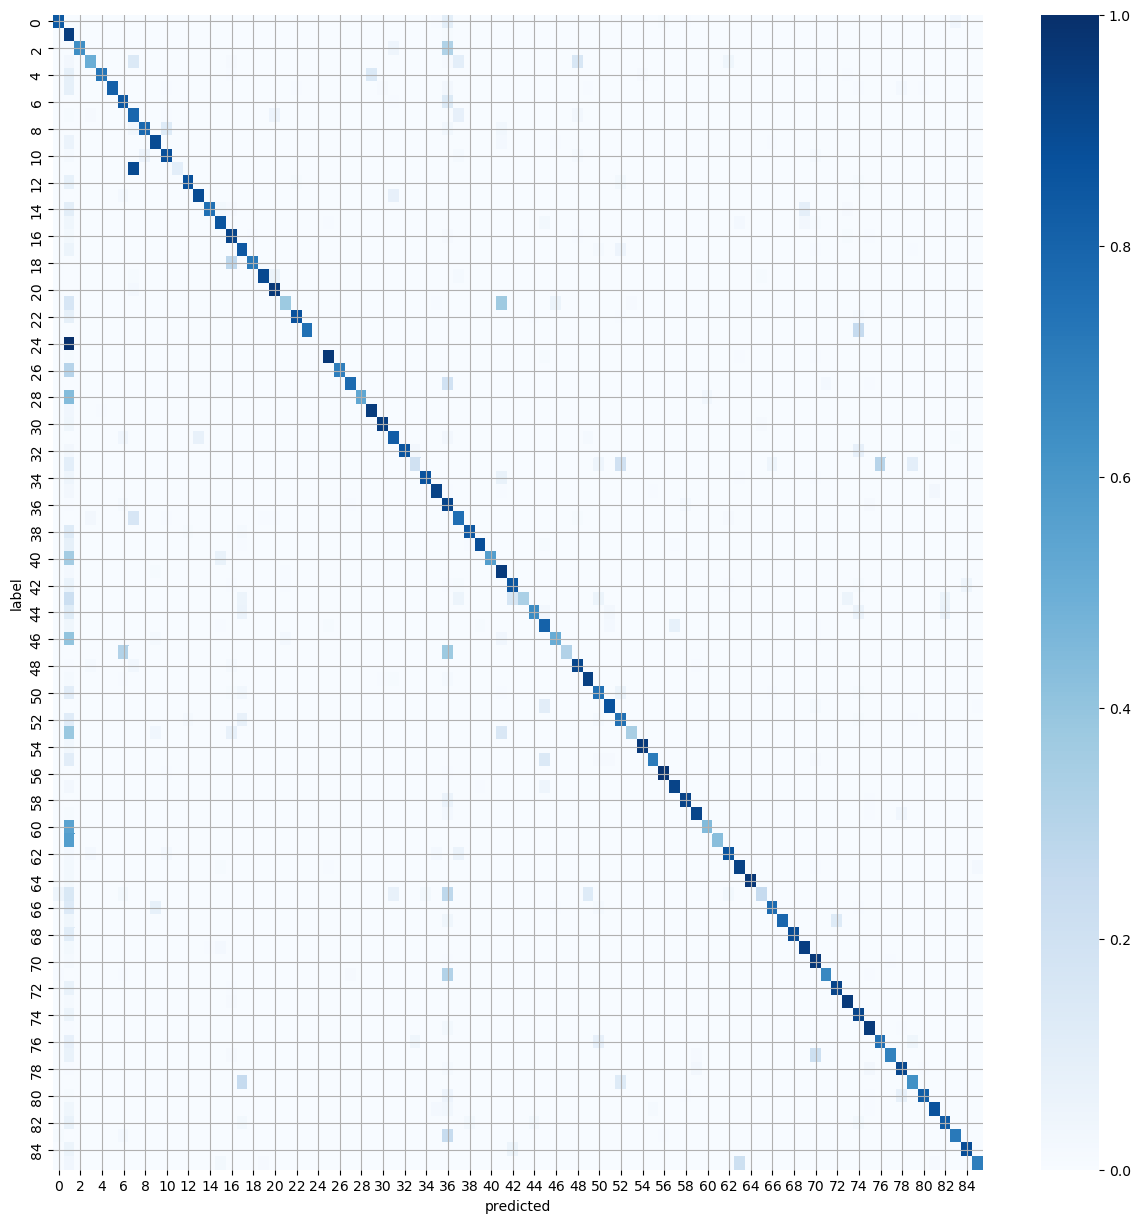
\includegraphics[width=0.18\columnwidth]{figs/confusion_matrix_MetzDreamDeep.png}&
		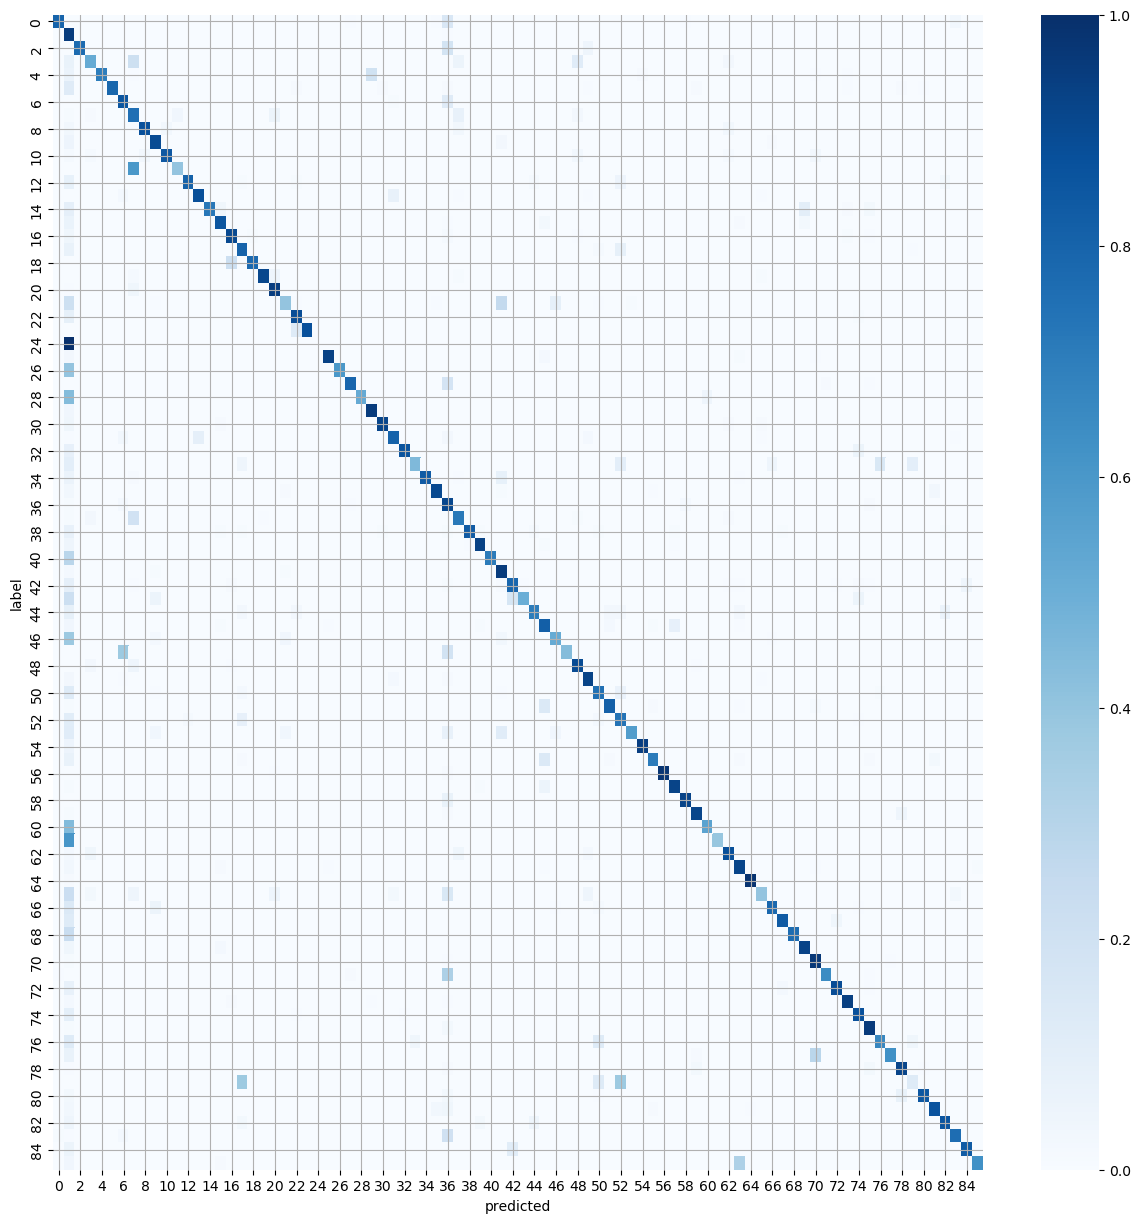
\includegraphics[width=0.18\columnwidth]{figs/confusion_matrix_voleursDhuile.png}&
		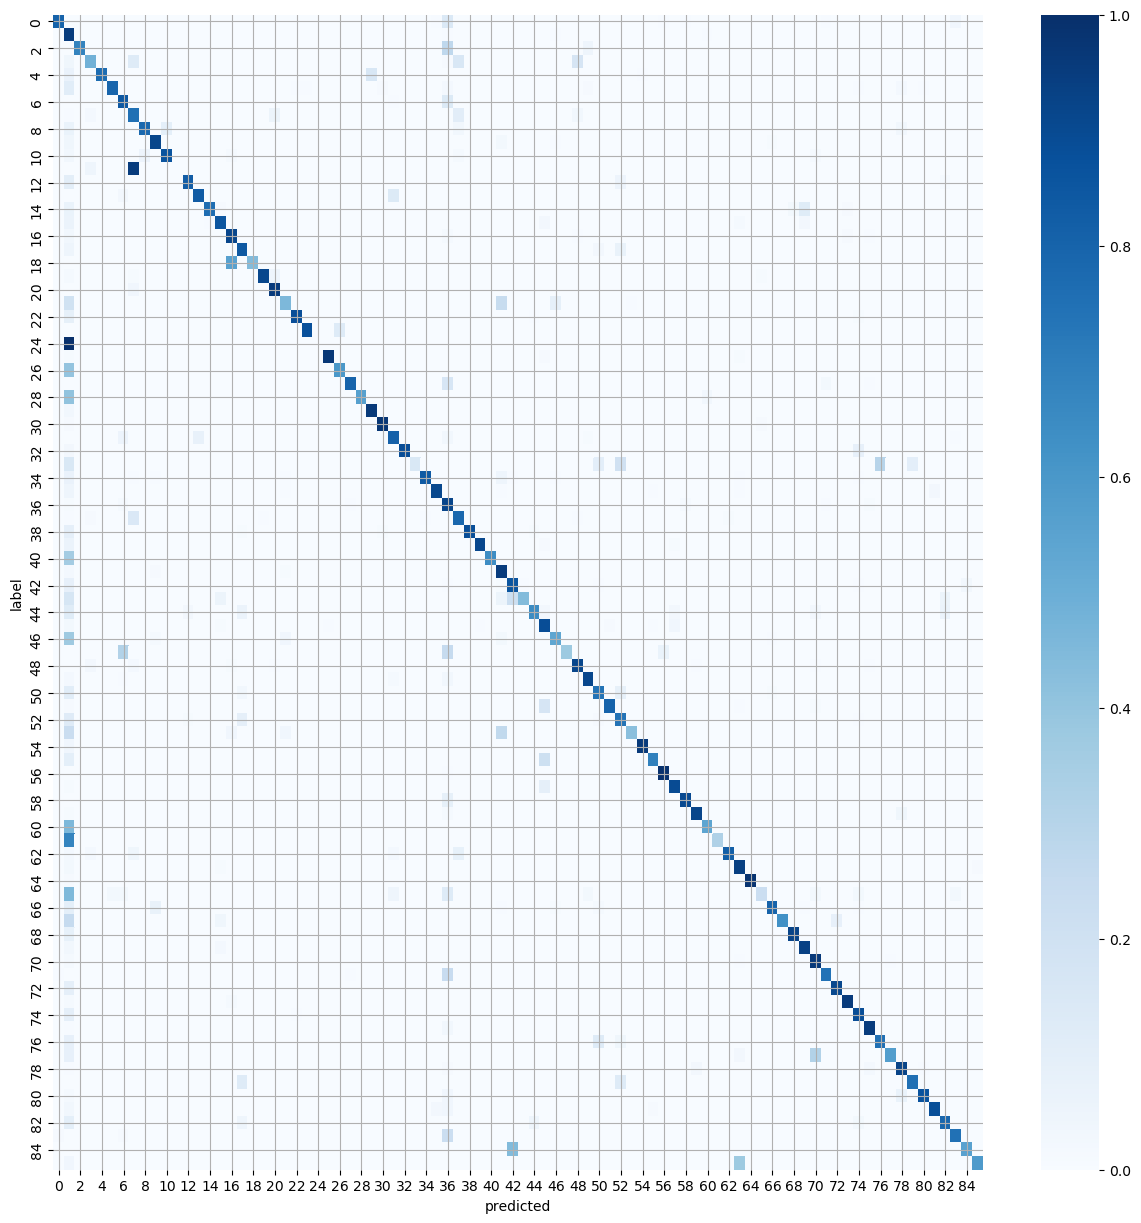
\includegraphics[width=0.18\columnwidth]{figs/confusion_matrix_JMBmc.png}&
		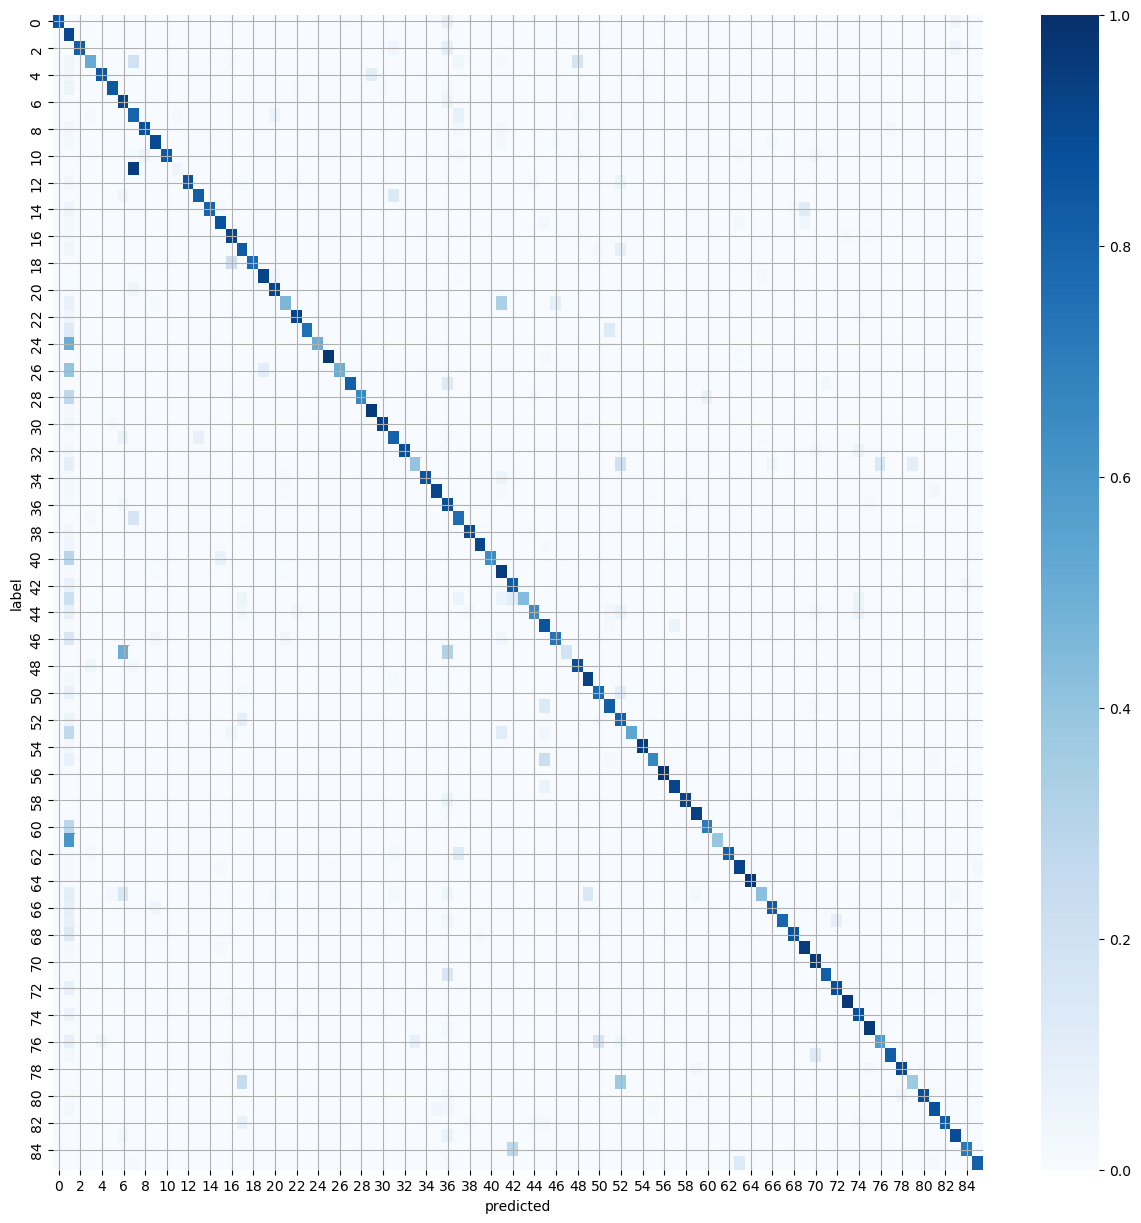
\includegraphics[width=0.18\columnwidth]{figs/confusion_matrix_AG0D.png}&
        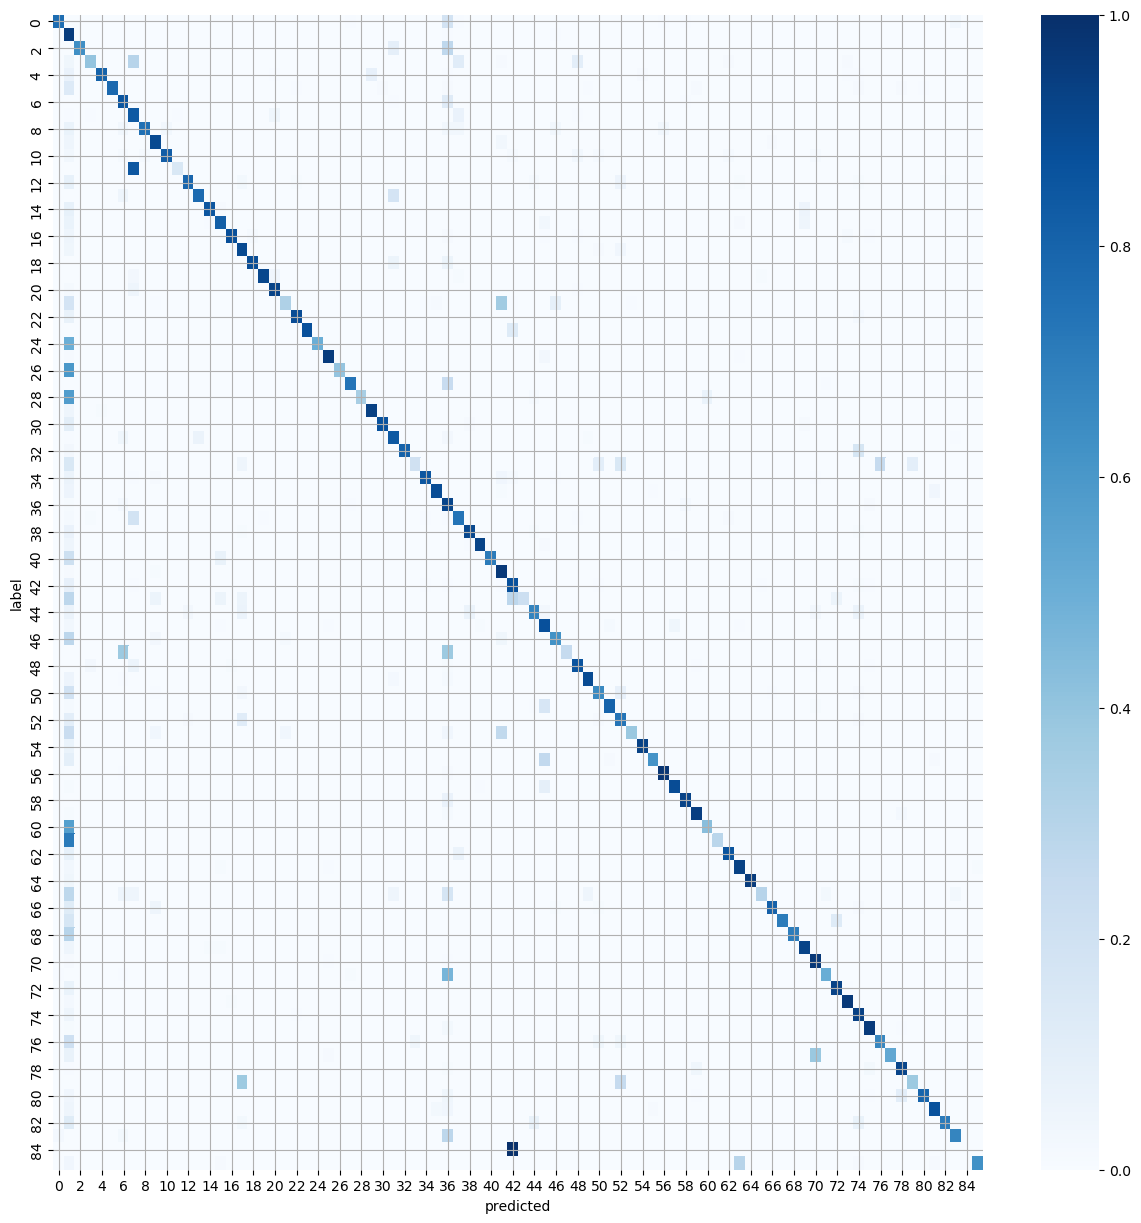
\includegraphics[width=0.18\columnwidth]{figs/confusion_matrix_ResMetz.png}\\
		Metz Dream Deep & Voleurs d'Huile & JMBmcfigs/ & AG0D\\
		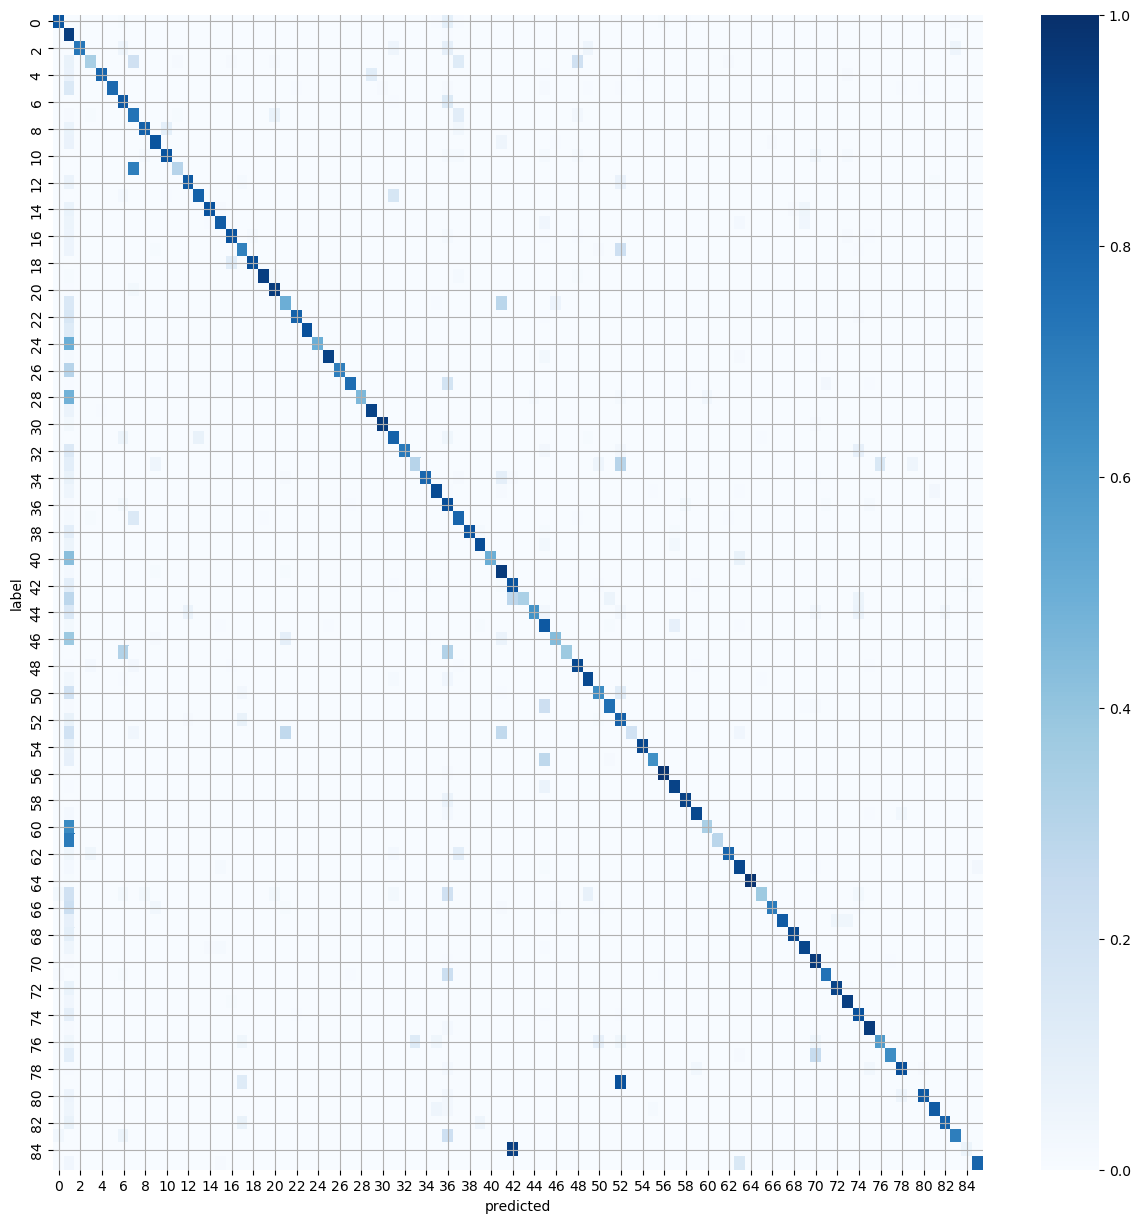
\includegraphics[width=0.18\columnwidth]{figs/confusion_matrix_CelestineFeuillat.png}&
		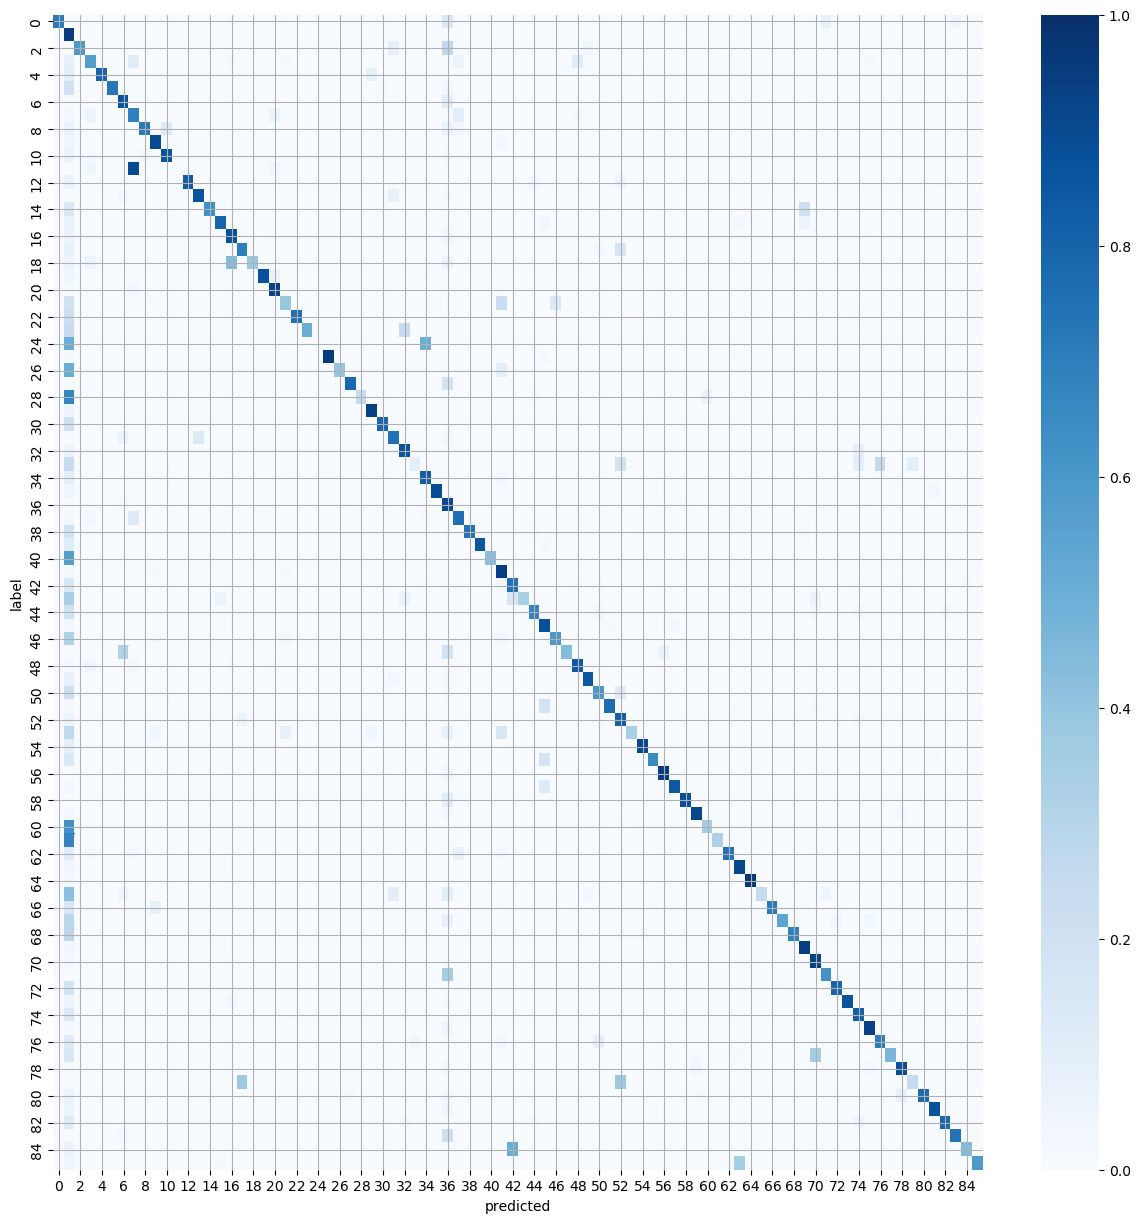
\includegraphics[width=0.18\columnwidth]{figs/confusion_matrix_LesJongleurs.png}&
		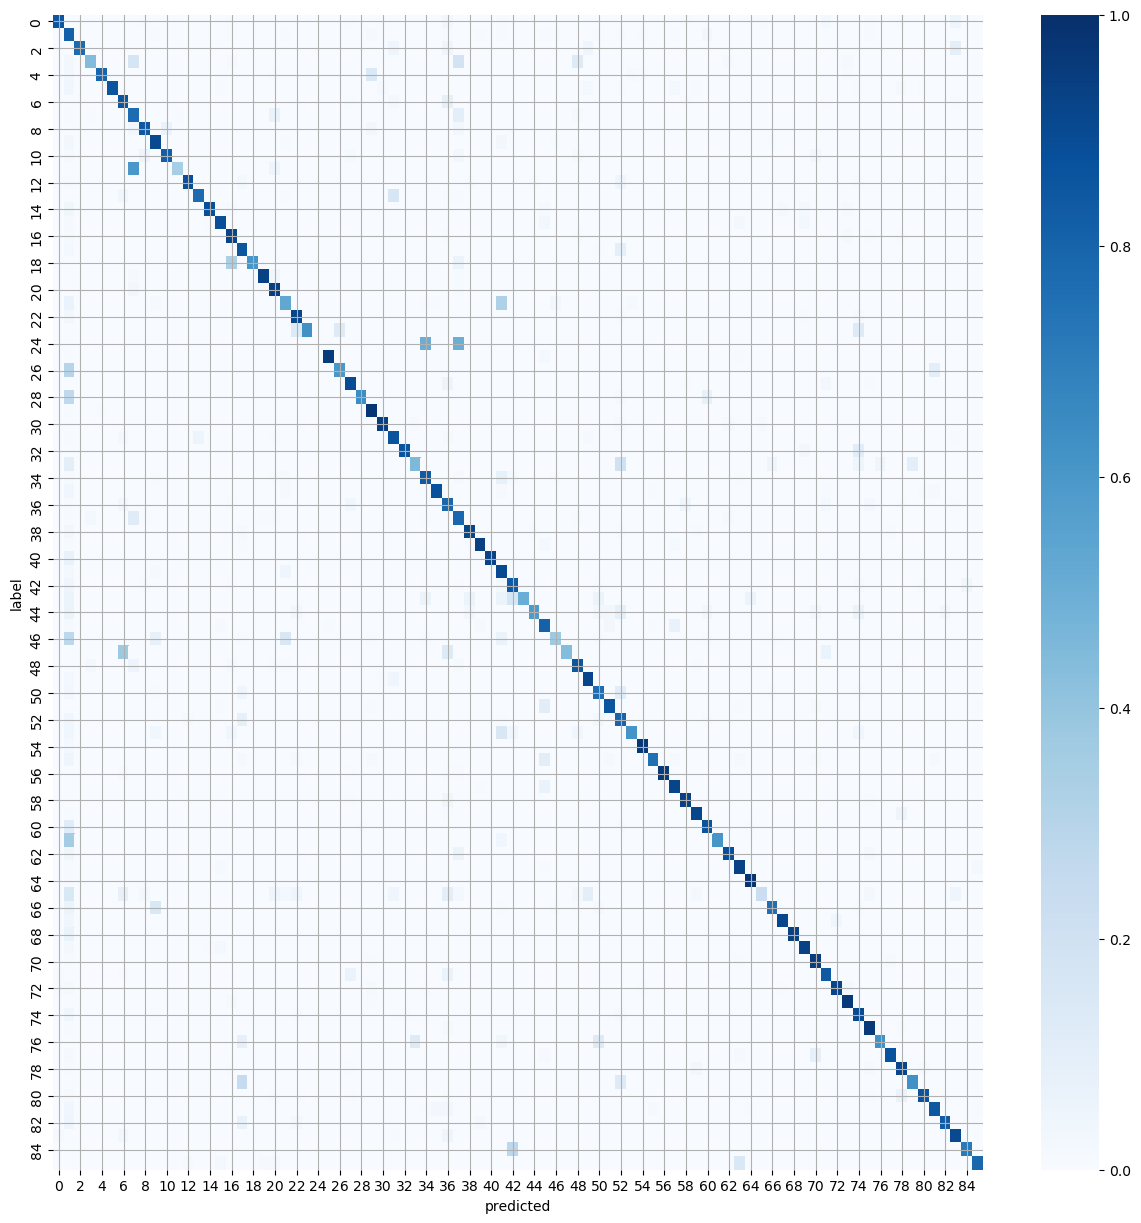
\includegraphics[width=0.18\columnwidth]{figs/confusion_matrix_DeepBeru'4s.png}&
		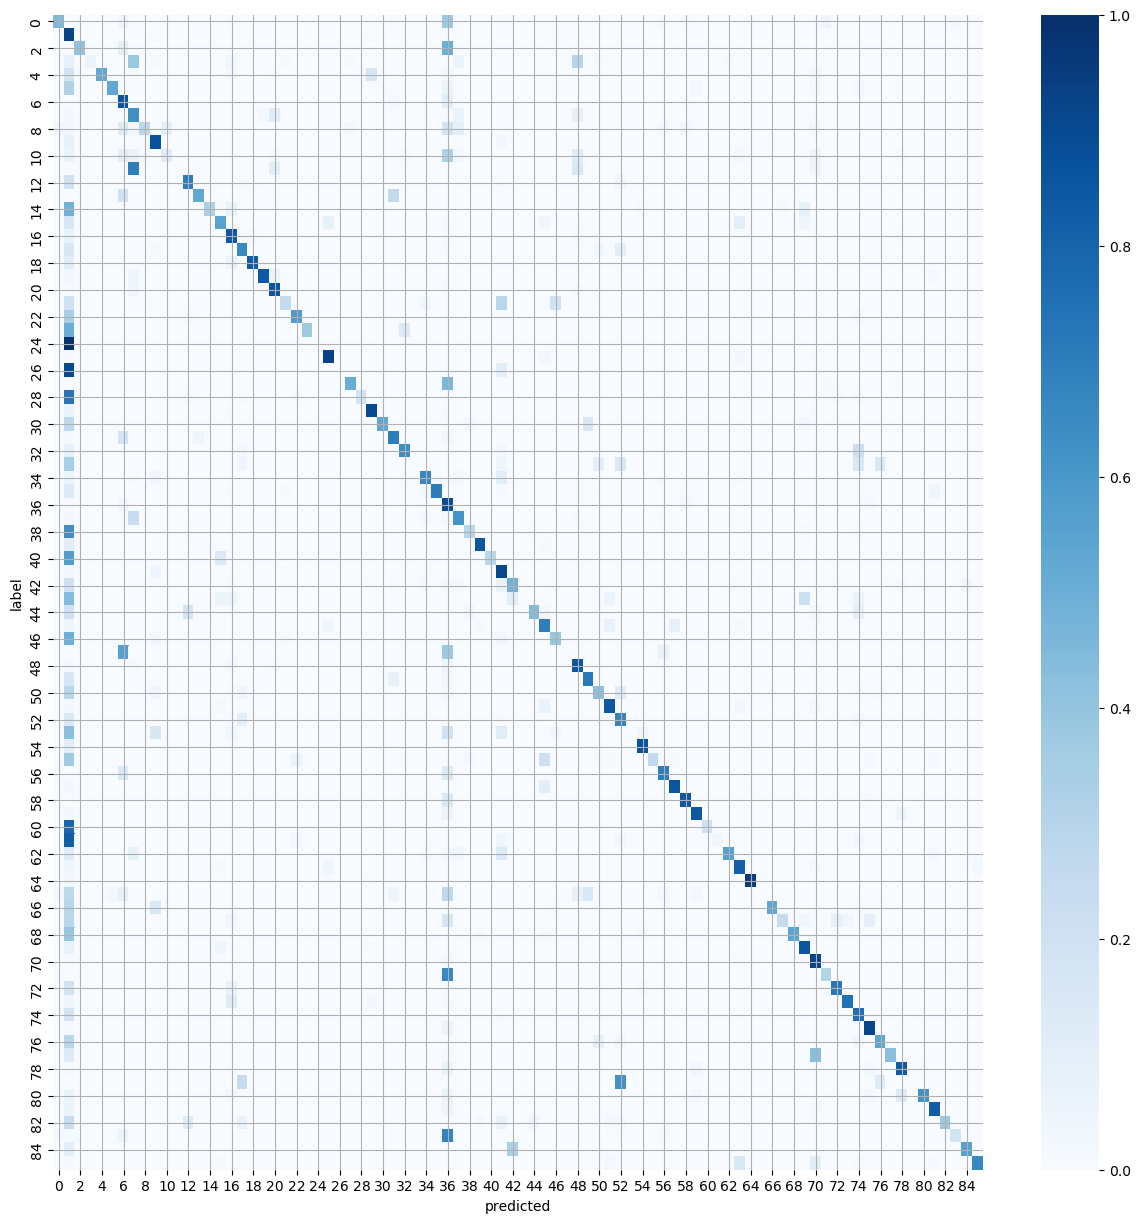
\includegraphics[width=0.18\columnwidth]{figs/confusion_matrix_TheWhaleSharks.png}&\\
		CelestineFeuillat & LesJongleurs & DeepBeru'4s & TheWhaleSharks & 
	\end{tabular}
	\caption{\label{fig:confusion} Confusion matrices of the best submissions of all the participants.}
\end{figure}


The confusion matrices allow to understand, when samples are misclassified, which are the most likely predicted classes.  Interestingly, the top ranking entries all share similar error patterns.

First, there is a tendency to misclassify as class 1 which is the detritus class, the majority class. Second, for the top ranking entries, when there is misclassification the misclassification is note widespread over all the classes but peaky on only few classes. Indeed, although this is hard to see from the plot, the confusion matrix is very sparse. 

Looking at the misclassification, it reveals that some of them would have been hard to prevent and it reveals an issue in the challenge preparation. For example, looking at the samples provided in appendix, the class 33 "Nectophore Abylopsitetragona" seems pretty similar to the class 52 "Nectophore Diphyidae".

%TODO : check why the off diagonal elements class do not match the badly classified classes listed above. There seems to be issues for class 11 for example ..


%-----------------------------------------------------------------------------------
\appendix

\section*{The distribution of samples per class}

The table below indicates the number of samples per class for each fold. The list is ordered from the most frequent to the least frequent classes.

% python3 plot_stats.py /opt/Datasets/ZooScan/train /opt/Datasets/ZooScan/derived.csv
\begin{tabular}{|c|r|c|c|c|}
Index & Name & Train & Public & Private\\
\hline1  & detritus & 243570& 13530& 13530\\
36  & Calanoida & 180000& 10000& 10000\\
75  & Oithonidae & 53387& 2965& 2965\\
58  & Acartiidae & 42096& 2338& 2338\\
41  & Chaetognatha & 33147& 1841& 1841\\
6  & Calanidae & 23797& 1322& 1322\\
29  & Evadne & 19225& 1067& 1066\\
9  & Oikopleuridae & 18457& 1025& 1025\\
69  & Phaeodaria & 15431& 857& 857\\
45  & egg  other & 14799& 822& 822\\
70  & Ostracoda & 12954& 719& 719\\
57  & Coscinodiscus & 12636& 702& 702\\
78  & Oncaeidae & 11490& 638& 638\\
63  & Limacinidae & 10038& 557& 557\\
59  & Corycaeidae & 10008& 555& 555\\
16  & nauplii  Crustacea & 8402& 466& 466\\
64  & cyphonaute & 8213& 456& 456\\
27  & Temoridae & 8200& 455& 455\\
74  & Salpida & 6996& 388& 388\\
54  & Penilia & 6368& 353& 353\\
39  & Noctiluca & 6056& 336& 336\\
7  & zoea  Decapoda & 5781& 321& 321\\
73  & nauplii  Cirripedia & 5604& 311& 311\\
15  & Foraminifera & 5570& 309& 309\\
52  & nectophore  Diphyidae & 5079& 282& 282\\
20  & Brachyura & 4764& 264& 264\\
46  & tail  Appendicularia & 4609& 255& 255\\
71  & Centropagidae & 4391& 243& 243\\
31  & Eucalanidae & 4213& 233& 233\\
49  & Haloptilus & 3983& 221& 221\\
25  & Bivalvia  Mollusca & 3916& 217& 217\\
48  & calyptopsis & 3900& 216& 216\\
37  & Decapoda & 3538& 196& 196\\
60  & artefact & 3465& 192& 192\\
22  & Doliolida & 3242& 180& 180\\
50  & eudoxie  Diphyidae & 3111& 172& 172\\
17  & gonophore  Diphyidae & 3060& 169& 169\\
21  & tail  Chaetognatha & 2825& 156& 156\\
80  & Harpacticoida & 2589& 143& 143\\
81  & Cavoliniidae & 2517& 139& 139\\
66  & Fritillariidae & 2314& 128& 128\\
42  & Annelida & 2085& 115& 115\\
83  & Euchaetidae & 2086& 115& 115\\
51  & egg  Actinopterygii & 1988& 110& 110\\
\hline
\end{tabular}

\begin{tabular}{|c|r|c|c|c|}
Index & Name & Train & Public & Private\\
\hline0  & Candaciidae & 1983& 110& 110\\
35  & Creseidae & 1869& 103& 103\\
34  & Actinopterygii & 1459& 81& 81\\
5  & Sapphirinidae & 1328& 73& 73\\
4  & Podon & 1326& 73& 73\\
72  & Ophiuroidea & 1285& 71& 71\\
56  & Pontellidae & 1289& 71& 71\\
13  & Rhincalanidae & 1210& 67& 67\\
38  & Obelia & 1091& 60& 60\\
12  & nectophore  Physonectae & 1045& 57& 57\\
19  & megalopa & 953& 52& 52\\
55  & egg  Cavolinia inflexa & 757& 42& 42\\
85  & Limacidae & 727& 40& 40\\
14  & Acantharea & 686& 38& 38\\
30  & Copilia & 686& 38& 38\\
3  & larvae  Crustacea & 638& 35& 35\\
77  & cypris & 632& 35& 35\\
68  & Neoceratium & 590& 32& 32\\
28  & scale & 576& 32& 32\\
10  & Hyperiidea & 536& 29& 29\\
62  & Luciferidae & 457& 25& 25\\
82  & Aglaura & 388& 21& 21\\
65  & part  Copepoda & 372& 20& 20\\
32  & Pyrosomatida & 336& 18& 18\\
44  & Rhopalonema & 308& 17& 17\\
8  & Gammaridea & 289& 16& 16\\
61  & cirrus & 269& 14& 14\\
53  & head & 244& 13& 13\\
76  & eudoxie  Abylopsis tetragona & 235& 12& 12\\
67  & Echinoidea & 234& 12& 12\\
2  & Calocalanus pavo & 214& 11& 11\\
33  & nectophore  Abylopsis tetragona & 188& 10& 10\\
11  & zoea  Galatheidae & 185& 10& 10\\
18  & metanauplii & 168& 9& 9\\
43  & larvae  Annelida & 170& 9& 9\\
84  & Tomopteridae & 172& 9& 9\\
47  & Euchirella & 156& 8& 8\\
40  & Spumellaria & 142& 7& 7\\
26  & ephyra & 98& 5& 5\\
79  & gonophore  Abylopsis tetragona & 88& 4& 4\\
23  & Scyphozoa & 78& 4& 4\\
24  & Ctenophora & 37& 1& 1\\
\hline
\end{tabular}


\pagebreak\newpage
\section*{Some examples for each class}

\begin{figure}[h]
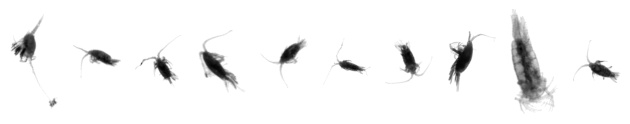
\includegraphics[width=\columnwidth]{collage/000_Candaciidae.jpg}\caption{Samples from the class Candaciidae }
\end{figure}
\begin{figure}[h]
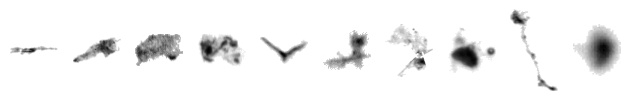
\includegraphics[width=\columnwidth]{collage/001_detritus.jpg}\caption{Samples from the class detritus }
\end{figure}
\begin{figure}[h]
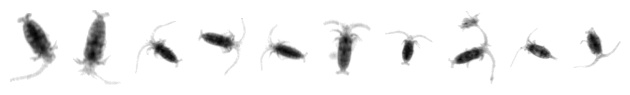
\includegraphics[width=\columnwidth]{collage/002_Calocalanus_pavo.jpg}\caption{Samples from the class Calocalanus pavo }
\end{figure}
\begin{figure}[h]
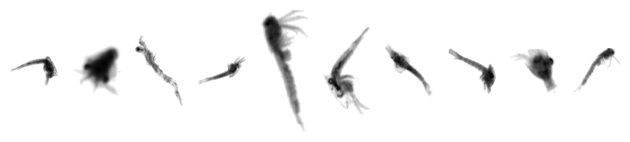
\includegraphics[width=\columnwidth]{collage/003_larvae__Crustacea.jpg}\caption{Samples from the class larvae  Crustacea }
\end{figure}
\begin{figure}[h]
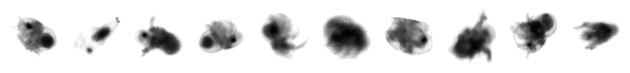
\includegraphics[width=\columnwidth]{collage/004_Podon.jpg}\caption{Samples from the class Podon }
\end{figure}
\begin{figure}[h]
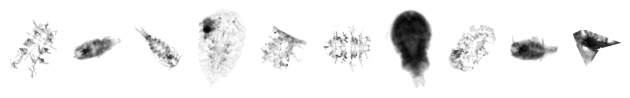
\includegraphics[width=\columnwidth]{collage/005_Sapphirinidae.jpg}\caption{Samples from the class Sapphirinidae }
\end{figure}
\begin{figure}[h]
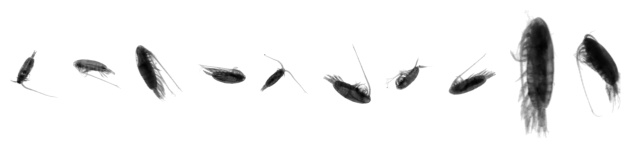
\includegraphics[width=\columnwidth]{collage/006_Calanidae.jpg}\caption{Samples from the class Calanidae }
\end{figure}
\begin{figure}[h]
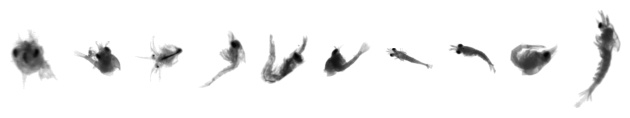
\includegraphics[width=\columnwidth]{collage/007_zoea__Decapoda.jpg}\caption{Samples from the class zoea  Decapoda }
\end{figure}
\begin{figure}[h]
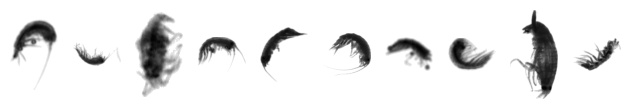
\includegraphics[width=\columnwidth]{collage/008_Gammaridea.jpg}\caption{Samples from the class Gammaridea }
\end{figure}
\begin{figure}[h]
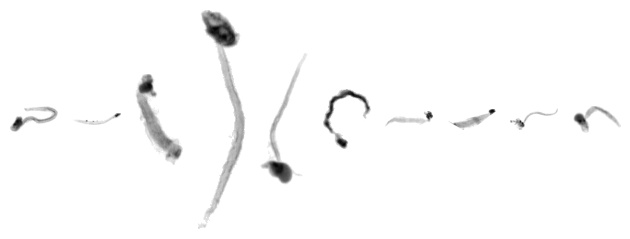
\includegraphics[width=\columnwidth]{collage/009_Oikopleuridae.jpg}\caption{Samples from the class Oikopleuridae }
\end{figure}
\begin{figure}[h]
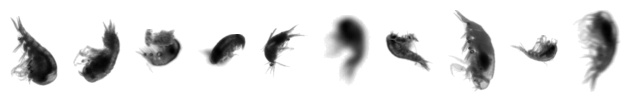
\includegraphics[width=\columnwidth]{collage/010_Hyperiidea.jpg}\caption{Samples from the class Hyperiidea }
\end{figure}
\begin{figure}[h]
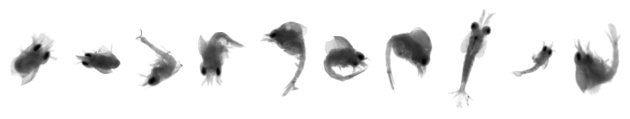
\includegraphics[width=\columnwidth]{collage/011_zoea__Galatheidae.jpg}\caption{Samples from the class zoea  Galatheidae }
\end{figure}
\begin{figure}[h]
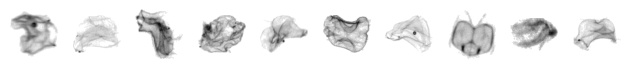
\includegraphics[width=\columnwidth]{collage/012_nectophore__Physonectae.jpg}\caption{Samples from the class nectophore  Physonectae }
\end{figure}
\begin{figure}[h]
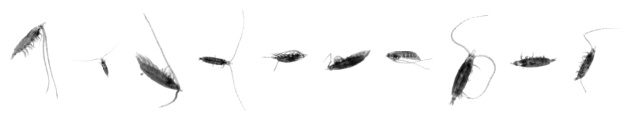
\includegraphics[width=\columnwidth]{collage/013_Rhincalanidae.jpg}\caption{Samples from the class Rhincalanidae }
\end{figure}
\begin{figure}[h]
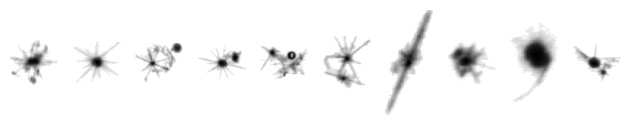
\includegraphics[width=\columnwidth]{collage/014_Acantharea.jpg}\caption{Samples from the class Acantharea }
\end{figure}
\begin{figure}[h]
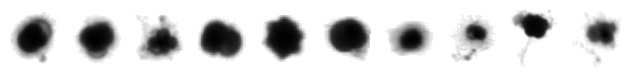
\includegraphics[width=\columnwidth]{collage/015_Foraminifera.jpg}\caption{Samples from the class Foraminifera }
\end{figure}
\begin{figure}[h]
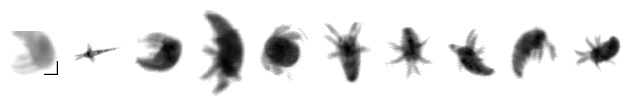
\includegraphics[width=\columnwidth]{collage/016_nauplii__Crustacea.jpg}\caption{Samples from the class nauplii  Crustacea }
\end{figure}
\begin{figure}[h]
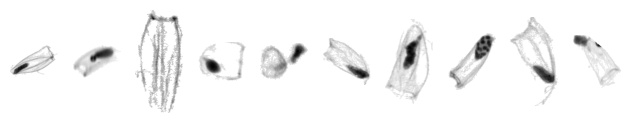
\includegraphics[width=\columnwidth]{collage/017_gonophore__Diphyidae.jpg}\caption{Samples from the class gonophore  Diphyidae }
\end{figure}
\begin{figure}[h]
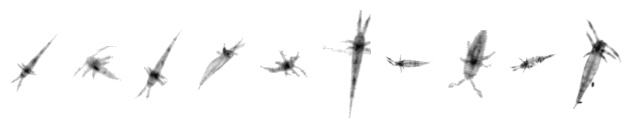
\includegraphics[width=\columnwidth]{collage/018_metanauplii.jpg}\caption{Samples from the class metanauplii }
\end{figure}
\begin{figure}[h]
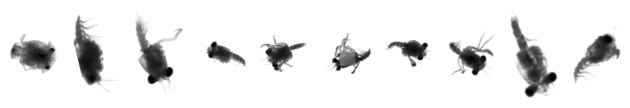
\includegraphics[width=\columnwidth]{collage/019_megalopa.jpg}\caption{Samples from the class megalopa }
\end{figure}
\begin{figure}[h]
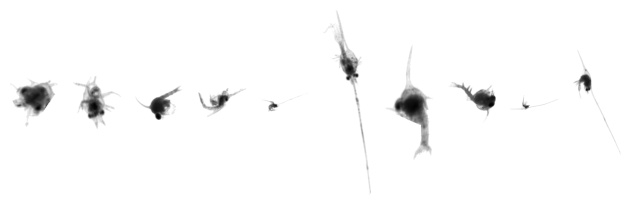
\includegraphics[width=\columnwidth]{collage/020_Brachyura.jpg}\caption{Samples from the class Brachyura }
\end{figure}
\begin{figure}[h]
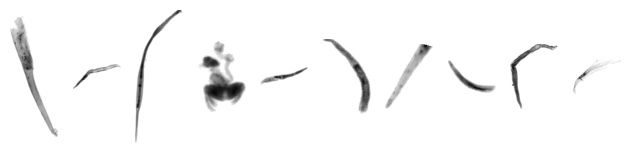
\includegraphics[width=\columnwidth]{collage/021_tail__Chaetognatha.jpg}\caption{Samples from the class tail  Chaetognatha }
\end{figure}
\begin{figure}[h]
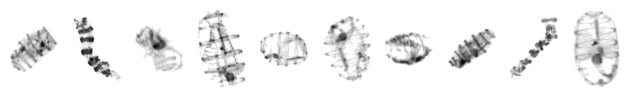
\includegraphics[width=\columnwidth]{collage/022_Doliolida.jpg}\caption{Samples from the class Doliolida }
\end{figure}
\begin{figure}[h]
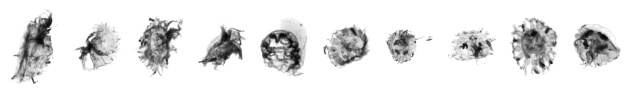
\includegraphics[width=\columnwidth]{collage/023_Scyphozoa.jpg}\caption{Samples from the class Scyphozoa }
\end{figure}
\begin{figure}[h]
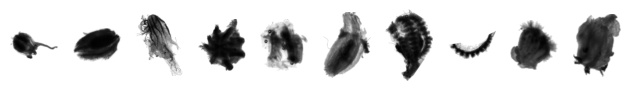
\includegraphics[width=\columnwidth]{collage/024_Ctenophora.jpg}\caption{Samples from the class Ctenophora }
\end{figure}
\begin{figure}[h]
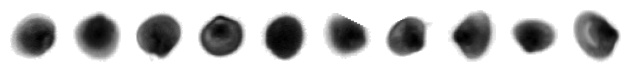
\includegraphics[width=\columnwidth]{collage/025_Bivalvia__Mollusca.jpg}\caption{Samples from the class Bivalvia  Mollusca }
\end{figure}
\begin{figure}[h]
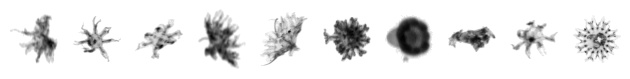
\includegraphics[width=\columnwidth]{collage/026_ephyra.jpg}\caption{Samples from the class ephyra }
\end{figure}
\begin{figure}[h]
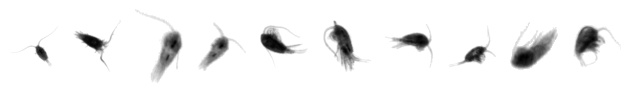
\includegraphics[width=\columnwidth]{collage/027_Temoridae.jpg}\caption{Samples from the class Temoridae }
\end{figure}
\begin{figure}[h]
\includegraphics[width=\columnwidth]{collage/028_scale.jpg}\caption{Samples from the class scale }
\end{figure}
\begin{figure}[h]
\includegraphics[width=\columnwidth]{collage/029_Evadne.jpg}\caption{Samples from the class Evadne }
\end{figure}
\begin{figure}[h]
\includegraphics[width=\columnwidth]{collage/030_Copilia.jpg}\caption{Samples from the class Copilia }
\end{figure}
\begin{figure}[h]
\includegraphics[width=\columnwidth]{collage/031_Eucalanidae.jpg}\caption{Samples from the class Eucalanidae }
\end{figure}
\begin{figure}[h]
\includegraphics[width=\columnwidth]{collage/032_Pyrosomatida.jpg}\caption{Samples from the class Pyrosomatida }
\end{figure}
\begin{figure}[h]
\includegraphics[width=\columnwidth]{collage/033_nectophore__Abylopsis_tetragona.jpg}\caption{Samples from the class nectophore  Abylopsis tetragona }
\end{figure}
\begin{figure}[h]
\includegraphics[width=\columnwidth]{collage/034_Actinopterygii.jpg}\caption{Samples from the class Actinopterygii }
\end{figure}
\begin{figure}[h]
\includegraphics[width=\columnwidth]{collage/035_Creseidae.jpg}\caption{Samples from the class Creseidae }
\end{figure}
\begin{figure}[h]
\includegraphics[width=\columnwidth]{collage/036_Calanoida.jpg}\caption{Samples from the class Calanoida }
\end{figure}
\begin{figure}[h]
\includegraphics[width=\columnwidth]{collage/037_Decapoda.jpg}\caption{Samples from the class Decapoda }
\end{figure}
\begin{figure}[h]
\includegraphics[width=\columnwidth]{collage/038_Obelia.jpg}\caption{Samples from the class Obelia }
\end{figure}
\begin{figure}[h]
\includegraphics[width=\columnwidth]{collage/039_Noctiluca.jpg}\caption{Samples from the class Noctiluca }
\end{figure}
\begin{figure}[h]
\includegraphics[width=\columnwidth]{collage/040_Spumellaria.jpg}\caption{Samples from the class Spumellaria }
\end{figure}
\begin{figure}[h]
\includegraphics[width=\columnwidth]{collage/041_Chaetognatha.jpg}\caption{Samples from the class Chaetognatha }
\end{figure}
\begin{figure}[h]
\includegraphics[width=\columnwidth]{collage/042_Annelida.jpg}\caption{Samples from the class Annelida }
\end{figure}
\begin{figure}[h]
\includegraphics[width=\columnwidth]{collage/043_larvae__Annelida.jpg}\caption{Samples from the class larvae  Annelida }
\end{figure}
\begin{figure}[h]
\includegraphics[width=\columnwidth]{collage/044_Rhopalonema.jpg}\caption{Samples from the class Rhopalonema }
\end{figure}
\begin{figure}[h]
\includegraphics[width=\columnwidth]{collage/045_egg__other.jpg}\caption{Samples from the class egg  other }
\end{figure}
\begin{figure}[h]
\includegraphics[width=\columnwidth]{collage/046_tail__Appendicularia.jpg}\caption{Samples from the class tail  Appendicularia }
\end{figure}
\begin{figure}[h]
\includegraphics[width=\columnwidth]{collage/047_Euchirella.jpg}\caption{Samples from the class Euchirella }
\end{figure}
\begin{figure}[h]
\includegraphics[width=\columnwidth]{collage/048_calyptopsis.jpg}\caption{Samples from the class calyptopsis }
\end{figure}
\begin{figure}[h]
\includegraphics[width=\columnwidth]{collage/049_Haloptilus.jpg}\caption{Samples from the class Haloptilus }
\end{figure}
\begin{figure}[h]
\includegraphics[width=\columnwidth]{collage/050_eudoxie__Diphyidae.jpg}\caption{Samples from the class eudoxie  Diphyidae }
\end{figure}
\begin{figure}[h]
\includegraphics[width=\columnwidth]{collage/051_egg__Actinopterygii.jpg}\caption{Samples from the class egg  Actinopterygii }
\end{figure}
\begin{figure}[h]
\includegraphics[width=\columnwidth]{collage/052_nectophore__Diphyidae.jpg}\caption{Samples from the class nectophore  Diphyidae }
\end{figure}
\begin{figure}[h]
\includegraphics[width=\columnwidth]{collage/053_head.jpg}\caption{Samples from the class head }
\end{figure}
\begin{figure}[h]
\includegraphics[width=\columnwidth]{collage/054_Penilia.jpg}\caption{Samples from the class Penilia }
\end{figure}
\begin{figure}[h]
\includegraphics[width=\columnwidth]{collage/055_egg__Cavolinia_inflexa.jpg}\caption{Samples from the class egg  Cavolinia inflexa }
\end{figure}
\begin{figure}[h]
\includegraphics[width=\columnwidth]{collage/056_Pontellidae.jpg}\caption{Samples from the class Pontellidae }
\end{figure}
\begin{figure}[h]
\includegraphics[width=\columnwidth]{collage/057_Coscinodiscus.jpg}\caption{Samples from the class Coscinodiscus }
\end{figure}
\begin{figure}[h]
\includegraphics[width=\columnwidth]{collage/058_Acartiidae.jpg}\caption{Samples from the class Acartiidae }
\end{figure}
\begin{figure}[h]
\includegraphics[width=\columnwidth]{collage/059_Corycaeidae.jpg}\caption{Samples from the class Corycaeidae }
\end{figure}
\begin{figure}[h]
\includegraphics[width=\columnwidth]{collage/060_artefact.jpg}\caption{Samples from the class artefact }
\end{figure}
\begin{figure}[h]
\includegraphics[width=\columnwidth]{collage/061_cirrus.jpg}\caption{Samples from the class cirrus }
\end{figure}
\begin{figure}[h]
\includegraphics[width=\columnwidth]{collage/062_Luciferidae.jpg}\caption{Samples from the class Luciferidae }
\end{figure}
\begin{figure}[h]
\includegraphics[width=\columnwidth]{collage/063_Limacinidae.jpg}\caption{Samples from the class Limacinidae }
\end{figure}
\begin{figure}[h]
\includegraphics[width=\columnwidth]{collage/064_cyphonaute.jpg}\caption{Samples from the class cyphonaute }
\end{figure}
\begin{figure}[h]
\includegraphics[width=\columnwidth]{collage/065_part__Copepoda.jpg}\caption{Samples from the class part  Copepoda }
\end{figure}
\begin{figure}[h]
\includegraphics[width=\columnwidth]{collage/066_Fritillariidae.jpg}\caption{Samples from the class Fritillariidae }
\end{figure}
\begin{figure}[h]
\includegraphics[width=\columnwidth]{collage/067_Echinoidea.jpg}\caption{Samples from the class Echinoidea }
\end{figure}
\begin{figure}[h]
\includegraphics[width=\columnwidth]{collage/068_Neoceratium.jpg}\caption{Samples from the class Neoceratium }
\end{figure}
\begin{figure}[h]
\includegraphics[width=\columnwidth]{collage/069_Phaeodaria.jpg}\caption{Samples from the class Phaeodaria }
\end{figure}
\begin{figure}[h]
\includegraphics[width=\columnwidth]{collage/070_Ostracoda.jpg}\caption{Samples from the class Ostracoda }
\end{figure}
\begin{figure}[h]
\includegraphics[width=\columnwidth]{collage/071_Centropagidae.jpg}\caption{Samples from the class Centropagidae }
\end{figure}
\begin{figure}[h]
\includegraphics[width=\columnwidth]{collage/072_Ophiuroidea.jpg}\caption{Samples from the class Ophiuroidea }
\end{figure}
\begin{figure}[h]
\includegraphics[width=\columnwidth]{collage/073_nauplii__Cirripedia.jpg}\caption{Samples from the class nauplii  Cirripedia }
\end{figure}
\begin{figure}[h]
\includegraphics[width=\columnwidth]{collage/074_Salpida.jpg}\caption{Samples from the class Salpida }
\end{figure}
\begin{figure}[h]
\includegraphics[width=\columnwidth]{collage/075_Oithonidae.jpg}\caption{Samples from the class Oithonidae }
\end{figure}
\begin{figure}[h]
\includegraphics[width=\columnwidth]{collage/076_eudoxie__Abylopsis_tetragona.jpg}\caption{Samples from the class eudoxie  Abylopsis tetragona }
\end{figure}
\begin{figure}[h]
\includegraphics[width=\columnwidth]{collage/077_cypris.jpg}\caption{Samples from the class cypris }
\end{figure}
\begin{figure}[h]
\includegraphics[width=\columnwidth]{collage/078_Oncaeidae.jpg}\caption{Samples from the class Oncaeidae }
\end{figure}
\begin{figure}[h]
\includegraphics[width=\columnwidth]{collage/079_gonophore__Abylopsis_tetragona.jpg}\caption{Samples from the class gonophore  Abylopsis tetragona }
\end{figure}
\begin{figure}[h]
\includegraphics[width=\columnwidth]{collage/080_Harpacticoida.jpg}\caption{Samples from the class Harpacticoida }
\end{figure}
\begin{figure}[h]
\includegraphics[width=\columnwidth]{collage/081_Cavoliniidae.jpg}\caption{Samples from the class Cavoliniidae }
\end{figure}
\begin{figure}[h]
\includegraphics[width=\columnwidth]{collage/082_Aglaura.jpg}\caption{Samples from the class Aglaura }
\end{figure}
\begin{figure}[h]
\includegraphics[width=\columnwidth]{collage/083_Euchaetidae.jpg}\caption{Samples from the class Euchaetidae }
\end{figure}
\begin{figure}[h]
\includegraphics[width=\columnwidth]{collage/084_Tomopteridae.jpg}\caption{Samples from the class Tomopteridae }
\end{figure}
\begin{figure}[h]
\includegraphics[width=\columnwidth]{collage/085_Limacidae.jpg}\caption{Samples from the class Limacidae }
\end{figure}


\end{document}
